%
% ``The Linux System Administrators' Guide''
%   by Lars Wirzeniu <liw@iki.fi>
%
% This is the top level LaTeX2e source code file for the book.  You should
% first create the files for the figures, then run this file through
% LaTeX2e (note that no versions of LaTeX 2.09 will work).
%
% If you have any problems with formatting or content, send mail to the
% author.
%
% If you like the book, please don't hesitate to send a post card.  Or
% even just an e-mail.  This project doesn't progress very quickly, but
% it _is_ fuelled by positive feedback and constructive criticism.
%

%
% Pick one of the following (make sure all but one have % at the front
% of the line)
%

% - single sided, letter paper (this should be the distribution default,
%   but only because 200 million americans complain to me if I make A4
%   the default paper size)
\documentclass{article}

% - single sided, A4 paper
% \documentclass[a4paper]{report}

% - double sided, letter paper
% \documentclass{book}

% - double sided, A4 paper
% \documentclass[a4paper]{book}


%
% You shouldn't need to touch anything after this line.
%

%\usepackage{linuxdoc}
\usepackage{graphics}
%\usepackage{html}
%\usepackage[html,3.2]{tex4ht}
\usepackage{makeidx}
\usepackage{showidx}
%\usepackage{t1enc} % anything for a good quote...


\makeindex

%
% Commands to mark various words.
%
%\newcommand{\defin}[1]{\textbf{#1}}	% a definition of a word or concept
%\newcommand{\cmd}[1]{\texttt{#1}}
%					% a shell command
%\newcommand{\fn}[1]{\texttt{#1}}
%					% a filename
%\newcommand{\man}[1]{\emph{#1}}
%					% a manual page
%					% don't include (1) in arg!
%\newcommand{\intnote}[1]{\footnote{\textbf{���ͦ��� �����������:} {#1} \textbf{(-�.�.)}}}
					% footnote of translator
\newcommand{\defin}[1]{\textbf{#1}}	% a definition of a word or concept
\newcommand{\cmd}[1]{\texttt{#1}\index{#1}}
					% a shell command
\newcommand{\fn}[1]{\texttt{#1}\index{#1}}
					% a filename
\newcommand{\man}[1]{\emph{#1}\index{#1}}
					% a manual page
					% don't include (1) in arg!
\newcommand{\intnote}[1]{\footnote{\textbf{���ͦ��� �����������:} {#1}\index{#1} \textbf{(-�.�.)}}}
					% footnote of translator

%
% \begin{verse}\it...\rm\end{verse} is used at the beginning of a 
% chapter to typeset a quote nicely.
%
\newenvironment{chapterquote}%
	{\begin{raggedleft}\it}%
	{\end{raggedleft}\vspace{2em}}

%
% \meta is used to mark comments inserted by the author.
%
\newcommand{\meta}{\large\textbf{META:\ }}

%
% We now begin the actual document.  Have a nice read.
%
\begin{document}

%--------------------------------------------------------------------
%\chapter[��Ӧ� �������æ�]{������������ ���˦� �� ����� ��Ӧ�� �������æ�}
\chapter{������������ ���˦� �� ����� ��Ӧ�� �������æ�}
%--------------------------------------------------------------------

        \begin{verse}\it
	�� ������� ����� ����� ������ �� ���˦������Ԧ.\\
        \rm\end{verse}

% the following metas need too much work for the next version
%
%	\meta copying a directory/disk verbatim
%
%	\meta disaster recovery: program to scan for ext2 superblocks
%
%	\meta explain lost+found; how to fix a filesystem; what to do when
%	there is a bad block; identifying the file that has the bad block
%	
%	\meta chart that shows characteristics of various fs: max size,
%	max file size, usable as root, max name length, speed, support
%
%	\meta 
%	Recovering from a bad MBR or super block.
%	Manually remounting (ro->rw, rw->ro, when, why)
%	automounting
%	MD patches
%	Why does Linux read/write disk in background?
%	how to mount a dos disk so that everyone can access it?
%	supermount
%	ide disks map away bad sectors (until they're too many, then
%	use badblocks)
%	mounting: mountee root becomes mount point, e.g. permissions/ownership
%	linux has maximum of 15 partitions (not inherent in partition
%		scheme!)
%	max ext2 part size is 2TB, file 2 GB
%	ext2 fragmentation
%	list important device files for disks et al as a table

        \noindent
	��� �������æ �� ��������Φ ������� ��� ���������� ����������
	������ ������ ��Φ����æ� � ������ �������. �� ��� ���Ҧ���
	�������� �����צ ������� ����� �����, ��� ����� ���� ���Ҧ����
	���Ҧ�Φ ����� � �������� ����Ȧ���� ����Ԧ� ��� Ҧ�����Φ����
	������ �������. 

	��� ���Ħ� ������� �Ӧ æ �������צ Ħ�. � ¦�����Ԧ �����˦�
	��� ����, �� ���� ������� ����������� � ���������, ��� ��
	���Ҧ��� ��������� ����� �Ӧ Ԧ � ��ͦ ����� �����, �Ҧ� Ȧ��
	��, �� ��� ����������Φ ������� ���˦�. ��� ��� ���Ҧ��� ����
	����������� �� ����� ���Ħ��, ���� �� ������� ��צ ����� ��
	�������, �� ������ ����� �������� ������������� ���������
	��������.

	�����Φ ����ަ ��� ��ͦΦ�������Φ ���˦� ��˦:
	%%
        \begin{itemize}
        \item

	������������ �����. ��� ��������� ���� �� ������, �� �����
	���Ц ����������� Ҧ�����Φ�Φ �����, ��˦, �� ���������,
	����צ��� ��������� ���˦� �����. (� ����� ��� ��� ¦�����Ԧ
	���˦� ������������ �� ���Ҧ���.)

        \item

	�������� ����� �� ���Ħ��. ���� ���Ҧ��� ���Ħ���� �� ����ͦ
	Ц����Ħ�� � ���� �������, ���� ����Ȧ��� ��Ħ���� ����Ԧ� ���
	Ҧ���� ��Ħ� Ħ������Ԧ, �˦ (���� Ħ������Ԧ) �� �����Φ
	�������� ���� ������. ����� � �����Ħ� ��� ���Ħ�� ����� ����
	���� ������� ���������� ˦���� �����æ���� ������ �� ������
	�����. ����� - ������� ������� �� ������ ���Ħ̦ Ԧ �����, ��
	�� צ��������� �� �����������������, � ����� ����������
	������������ ����� �� ��� �������� ������� צ� ��æ������ �����.

        \item

	��������� ������ϧ ������� (���Ҧ����� ����) �� �������
	�������� � ���Ħ̦� �����. ���� �� ������� ��������� Φ����
	��� ������ �� ���� ����, ���� �� ����� �� �������� �������
	�������. \begin{intnote}�Ҧ�, Ȧ�� �� ����-��������, ���� � ��������
	�Φ���� �� ������� צ� ���������� ��ͦΦ�������� ���������
	Φ���� Ħ�. �Φ�� ���� ������������� ����-��������� ����� �
	Ц��� ����, �� ��������� ���Ħ� �����. � ����Ӧ ��������
	����� �������� ������� \cmd{mkswap}, ��� �������� "<�������
	�������">. �������Ħ ����� �����դ � ��������� ����-���Ħ��
	Ԧ���� ���æ������ Ц����\intnote{sign�ture}, � ������դ����
	���-���� "<�����"> Ц����Ħ���.\end{intnote} ���� ����� ����� ����������
	����� �� ���������� �� ���.

        \item 
	
	���������� Ҧ���� �������� ������, ��� ���������� �����
	��������� (��� �����������, ��� � ������, Ԧ���� ��Ħ, ���� ��
	����Ȧ���. ������ ��������Φ �����צ ������� � ¦�����Ԧ
	�����˦� ���Ҧ��� � �������������� ����� ������.).

        \end{itemize}

	� ���Ħ̦~\ref{chap:mem} ͦ������� �������æ� ��� צ��������
	���'��� �� �������� ���, ��� �˦ ��� ����� ���� ����� �������,
	��� ����������Φ �������.

	����� ���Ħ� �������, �� ��� ���Ҧ��� ����� ��� ����˦ ��
        ����˦ �����, CD-ROM �� ������� ���Φ��ϧ ��Ҧ���. 

\section{��� ���� ������ϧ�}

	�Φ��, � ����� � �����, ���Ҧ������ ��� צ�ͦ���� ͦ� �����
	���� ������ϧ�: ����Φ ������ϧ � ��צ�����
	��������\intnote{random access} (����� � �����) �� ������ϧ �
	������������ ��������\intnote{character devices} (����������
	���� � ���Φ�Φ ��Ҧ��� �� ���̦���Φ ̦Φ� ��'����), ���˦ �
	���� ������ ���� � ���̦������ ��������, � ��ۦ - �
	��צ�����. ����� �����Ҧ�, ���� Ц�����դ���� ��������,
	������������� � �����צ� �����ͦ \defin{���æ������ ������
	��������}. �� ��� ������� �� ������ � ���� ��������, ��Φ
	��������� �� צ������������ �� �������� ��������������
	���æ������ ������. ����� ����� �� ���Ҧ�Φ ���Φ ���æ���Φ
	�������� (��� � �˦�� ���æ���Φ �������ϭ�� �������������,
	��, ���������, �������� ������Φ� �� ���������� ���̦�������
	�����) ��� ���� Ԧ����, ��� ���������� �� ������ϧ�.
	���������, ��� ����, ��� ������ צ�������� ���� �� �������,
	��������� ������ ��������

		%
		\begin{quote}\tt
\verb|$| {\sl cat filename $>$ /dev/lp1} \\ 
\verb|$|
		\rm\end{quote}
		%

	� �ͦ�� ����� ���� ������������� �� ������Ҧ (�������� � ����
	������� ���� � �����Ԧ �����ͦ���� ��� ��������). �����,
	�������� �� ��, �� ����� ������� ������ ������� �����������
	����� ����� �� ������� ������ ������� ������������, ����
	������ ������������ �������� ��������� ��� ����� (�
	¦�����Ԧ ������ \cmd{lpr}). �� �������� ������դ, �� Ԧ����
	���� ���� ����������� �� ������� ��� ����� � ����� ������ ����
	� ����������� ������� �� ���� ���������, �� Ԧ���� ����������
	� ����������� ������������. ���� ��Ħ��� ���Ҧ��� ����� ���
	¦�����Ԧ ����� ������ϧ� � �����ͦ. �����Ħ, ���������ަ ��
	�����Φ ����������� ��� �˦�� ��� "<������ϧ"> ��������� Φ����.

	����� ��, �� ������ϧ � ���������� ������� � �����צ� �����ͦ
	(� �������Ҧ� \fn{/dev}, ���� ����� ������ ���������� �˦ �
	������ϧ� ������� �� ��������� ������� \cmd{ls} �� ����-��ϧ
	���ϧ Ц������ϧ �������. ������ �������� �� ����Φ ���
	�������Φ ������� \cmd{ls -l} ͦ����� ��� ����� �� ������� ��
	��� ����. ���������, ��������� �� �������� ����
	���̦������� ����� �� ��ϧ� �����ͦ � ����:
		%
		\begin{quote}\tt
\verb|$| {\sl ls -l /dev/cua0} \\
\verb|crw-rw-rw-   1 root     uucp       5,  64 Nov 30  1993 /dev/cua0| \\
\verb|$| 
		\rm\end{quote}
		%

	����� ̦���� � ������� ��������, ����� `{\tt c}' �
	�������������� ������Ħ  � {\tt crw-rw-rw-} �����դ ���˦�������
	�����������צ ��� �����, �����, � ����� �������, ����������
	���æ������ ����. ��� ��������� ���̦� ��� ������ ���� `{\tt
	-}', ��� �������Ҧ� - `{\tt d}', � ��� ������� ������ϧ� -
	`{\tt b}'. �������� �������æ� ������ � ����� ������� �
	���Ҧ�æ Ц������ ��� \cmd{ls}.

	��������, �� ��צ�� ���� ������ϧ �� ���������Φ �� ������
	����'���Ҧ, ����� ���æ������ ������ϧ� �������
	���-����. ����, ��, �� �� ����� ���� \fn{/dev/sda}, �� ��
	�צ����� ��� ��, �� �� �����Ħ ����� SCSI ���� Ц��������� ��
	�������. ���Ҧ����� �Ӧ� ��� ������ϧ� � �����ͦ ������ ������
	�������� ��������� ����� ����Ԧ���� � צ� ����� ���� ������
	��������� ������ ���������� (�� ���Ҧ��� צ����������� צ�Φ
	��������� ��� ���������� �������� �� ���������� ���æ���Φ
	����� ��� �����).

\section{�����˦ �����}

	����� Ц����Ħ� ���������� ������ � ���ͦ���ϭ���, �� ���
	צ�������� �� �������� ���˦�. ���� �� ��� �����ͦ � ���ͦ����
	�� ��������, �� ������ ���������� ����. 

	�������~\ref{fig:hd-schematic} �����դ ���������� Ħ������
	��������צ��� ������ ��������� �����. �������� ����
	����������� � ��Φ�� ��� ¦���� �����������
	\defin{�������}\footnote{�������� �������������� � �����ϧ
	��������, ���ϧ, �� ���ͦΦ�, �צ��� � �������� �����
	��������� �����} �� ���� ���� ��� ����צ \defin{������Φ}
	�����Ԧ ���Φ���� ���������, ��� � ����������դ���� ��� ������
	�����. ��� ����ϧ ���ϧ ������Φ ���դ ������
	\defin{���������-צ��������� �������}, ��� ���̦�դ ��� �ͦ���
	������Φ �� ������Φ ��Φ. �Ӧ �������� ����������� ��
	�Ц��Φ� �Ӧ, ������ ����˦��� ��������� ������� 3600 ����Ԧ�
	�� �������, ��� ����� � ����� ���������� �����Φ��� ����� ��ݦ
	�������Ԧ. ������� ������ ������������ ������ ��Ħ��� �������,
	� ��� ���, �Ϥ������ � ���������� �������, ��� ��������
	�����צ��� ������� �� ����-��ϧ ������� �����.

	�������� (CPU) � �������� ���� ��������� �����
	\defin{�������� ���������}. �� �צ����� �Ӧ ��ۦ �������
	����'����� צ� ����Ȧ����Ԧ �����, �� ���� ������������� ���
	�� ����� ������, �� �����צ ���������� ������ �������������
	����� �����, ��� ���� ���� � ���-�� ��������� ��
	����'�����. ������� ������, ����'���� ������ ���� �������
	"<���, �����, ��� ��Φ ��, �� � ����">, ��ͦ��� ����, ���
	���������� ���Ǧ ���̦������Ԧ ����������� �����̦� Ԧ���� ���
	�������� ������� � צ���צ��� ��������� � ������ Ц��� �����,
	��� ���Ҧ��� ͦ��� ����� ������ Ц� �������
	�������. �������Ħ, ��������� �� ��������� ���������� ��� ��
	������ ������� �����, ��� ���-���� �������� ����Ԧ��, Φ� צ�
	ͦ� �� ����. �Ҧ� ����, ��������� ���� ������ ���˦ ��ۦ ��ަ,
	��˦, �� ��������� ��� ����������� ��ͦ�� ��������� �����Ҧ�.

	������Φ ���� ��Φ, ��������� ���, �� ����Ȧ��� �����
	��������-����Ӧ����� �����������צ ��� ����������. �Ҧ�
	��������� � �� æ�� �'���� �Ӧ����� ����� ����������, �����,
	�� ������, �� ������� ��������, ��������Φ ������, �˦ �������
	������� ����Φ���� ������, ��� ��� �� �� ��� צ�������� ��
	����ͦ��� ������Ц� ������ �������� ���˦�.

	���Φ�Φ ������Φ, �� ��������, ���Ħ��Φ �� ����������Φ
	˦����, �� ������ ����� \defin{��Ҧ���}, � æ � ���� �����
	��Ħ��Φ �� \defin{�������}. ����� ��Ħ� ����������դ���� ���
	���������� ��������� �� ������Φ ��������� ����� �� ���
	��Ħ����� צ������ �������� ��� ���̦�. ��� ��������� ���Ҧ���
	ͦ��� �� ����� �������� ������ "<�������� 3, ��Ҧ��� 5, ������
	7">. ������Ԧ�� ����� �����Ҧ� � ������ ��� �Ӧ� ��Ҧ��� ��
	�����, ��� ���˦ ����� ���Ħ����� ¦���� �����Ҧ� �� ���Φ�Φ
	��Ҧ��� (�Ӧ ������� ������ ���� � ������ ������� ���������
	Ʀ������ ���ͦ�, �, ����, ¦���� �����Ҧ� ��ͦ������� ��
	������� �� ���Φ������ ��������� ��Ҧ����). ������� ������ ���
	512~���� �����. ���� ��� �� ��¦ �� ���� ��������� ��'�����
	����� �������, Φ� ���ͦ� �������.

		\begin{figure}[thb]
		\begin{center}
		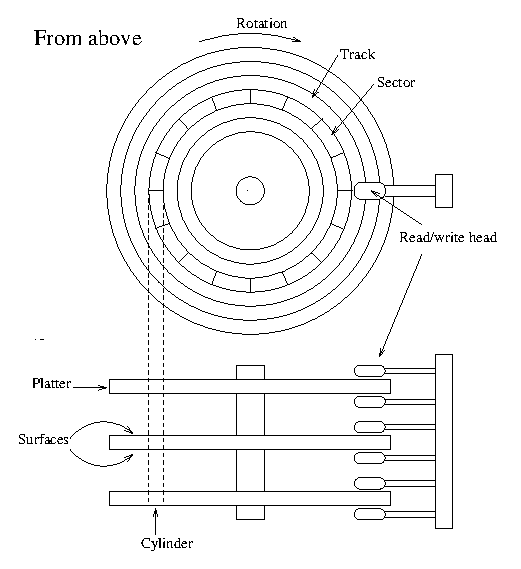
\includegraphics{disks/hd-schematic.ps}
		\end{center}
		\caption{���������� ���������� �������� ������ ��������� �����.}
		\label{fig:hd-schematic}
		\end{figure}

	����� �������� ����� ���Ħ���� �� ��Ҧ��� (� �������) ���
	����, �� � ��ۦ. �� ������� ��, ��, ���� ������� �� ��Φ� �
	��������� ����������� ��� ������ ��Ҧ����, �� ������� �� �Ӧ�
	����� ������� ��������� ����������� ��� ����� �
	���������. �Ӧ צ���צ�Φ ��Ҧ��� ����� ���Ԧ ���������
	\defin{��̦�����}. ����������� ������� � ��Φ�� ��Ҧ���
	(��̦����) �� ���ϧ ������ ������ ���. ����, ��Φ �����
	����������� ����� �����, ��� ��Φ, �� ���� ������ �������
	������������ ��������� (���������, ����), ��������������� �
	������ � ���� � ��̦��Ҧ. � ������ ��ڦ צ������ ����Ȧ�Φ���
	����������� ������� ��� �����Ц �� ��� ����� �, ����, ��
	Ц����դ ����˦��� ������. �� ������ �����Ѥ���� ��������
	����������� ����� ����� �����, � �����, �˦ �����������
	���������� ����������� �� ˦����� Ҧ���� Ʀ������ ���Ħ���
	����� ������ ����� \defin{��������������}.

	����� ���������, ��� ������� (��, �� ��Ԧ, � ����� � ��� ��),
	��̦��Ҧ� �� �����Ҧ� ���Ԥ�� צ�Ҧ��������\intnote{��� ��Φ��
	����̦ ����� �� ���ϧ, ��������, � �� � �����Ӧ
	������.}. �����Φ��� �Ӧ� ��� �������Ҧ� ���������
	\defin{������Ҧ��} ��������� �����. ������Ҧ� ����� �����
	�����դ���� � ���æ���Φ� ���'�Ԧ, �� �������� צ� ���������,
	� ������ ����� \defin{CMOS RAM}\begin{intnote}������� � ������������
	����æ צ���������, �� ��Ԧ, Ԧ���� �� PC-����Ӧ�. 

	����� ������Ҧ� ����� � CMOS � �����Ʀ���� ������� PC
	BIOS'��. ��ۦ ������� ������������ ¦��� ����������� ��������
	���������� ������Ҧ� ���˦�. ������ ��� ˦���� �̦� ���
	�������� - � SunOS �� Solaris � ���æ����� ���� ����� ��Ц�
	���˦�, � �˦� ��������� � צ���צ�Φ��� Ҧ�Φ ���� ���˦� ��
	�� ������Ҧ�. ��� ����� ������������ �������� � ���� ��������,
	��� �������� � ��������� ������ �����. Sparc ����� ��� ��
	������դ���� BIOS'�� ��� ���������� ������Ҧ� ���˦� � �ϧ
	�����ϧ �������, �� ����'����� Sun ������ �� ����� BIOS'��. �
	�� ����, �� ���� Sparc ����� �������� ������Ҧ� ���˦�, ����
	���� �����, ���� ����� � ��� ��Ħ������ ڦ ���� ��������.

	����� ¦��� �����Φ BIOS'� (��������� �Ӧ, �� ������������ ��
	������Φ�Φ� ���� - � �� ����Ҧ��� � �����Φ� ��� ����ϧ ���ϧ
	����������ϧ ����� PC ��� æ�� ���������) �ͦ��� ���������
	���� ���˦� Ц�'������� �� �������. � צ� ����������� ��
	����������� ������� �ͦ�� � ��������� BIOS'� Ц��� �ͦ��
	���˦�. 

	 \end{intnote}. � æ�� ���'�Ԧ �����æ��� ������� Ħ�������� ��� ���� Ц�
	��� ������ ������� ��� ������Ҧ�.

	�� ���� BIOS\footnote{BIOS - �� ����� �������� ��� �����������
	������ �������, ��� �����դ���� � ROM ����'�����. ����
	צ��������դ ���������� ����� ������� צ� ��������� ��������
	�� ���� �������, ���� �����̦��� ����������� �����æ�Φ�
	�����ͦ.}\intnote{(���. ROM)} ��� ���Φ ��������� �������Φ
	��� ����������Φ, ����� �˦ �����Ѥ���� ���������� ����������
	�� ��Ҧ���, ����� ���� ¦����� �� 1024 (����� ��������� ���
	����� � CMOS RAM), �� � ������� ����� ��� �������� ��������
	���˦�. ��� ������� ����� �� ���� ��������� ������������, ��
	צ� �� ���� ��������ϧ ������Ҧ� ����� � \defin{����������
	������}, �������Φ ���'������ � ��˦, �˦ ¦���� Ц������� ��
	�����ϧ �����æ�. ���������, �������� ���� ���� ���� 8
	�������, 2048 ��Ҧ��� � 35 �����Ҧ�\footnote{����� ����Φ
	�����}. ���� ��������� ���� ������ ����'����, �� צ� ��� 16
	�������, 1024 ��Ҧ��� � 35 �����Ҧ� �� ��Ҧ���, �� �����������
	����� ����� �����ϧ ��������ϧ ��֦ ��Ҧ��� � ��������
	������Φ ������ �� ����� �������� �� � ���, �� ��������� ����
	����'������. �������Ħ ���������� ������ ������ ����������
	���� ���� ������ ��������, �� ����� ������ ���� �� ������
	������� �� �����������, �� � ���������� ������Ħ (���, ����� �
	����, �� �� ��� צ�������� �� ���������� ����ͦ��� ��������
	������). ���� �������������� Ʀ������ ����� ��������� ��������
	������� ��� �������� ����Φ��æ� ���˦� � ������
	����������������� ������ ����ͦ��æ� �������Ԧ ������� ��
	������� ������������ ����� � ����� ������ ��̦����.
	
	� �������� �������������� ����� ���������� Ԧ���� IDE
	���˦�. SCSI ����� �������������� ���̦���Φ ������ �����Ҧ�
	(�����, ��������� ���������� ���̦������ ����� ������� �
	������� "<�������-��̦���-������">) � ���Ӧ� ����� ����� ���
	�Ц�������� � ����������, ���� ���� ���Φ��� ��������Φ צ�
	������ϧ ��������. ���ͦ����, �����, �� � � ������� �� SCSI
	������� ����'���� ����� ���� �� ����� ��������ϧ ������Ҧ�
	�����.

	����� ��, �� ����� ����� �� ��� � ���������� ������� ���
	�������� ������Ҧ� �����, צ� ��צ�� � �� ����� ��ͦ�����
	�˦�� ��Φ � ����� ������ ��̦����. ��ͦ��� ����� צ�
	����������� ��������� ������� ����� ���̦���Φ �������, � �� �
	��������Ԧ ��� ��������� ����� �� ������ � ��Ӧ. �� ��������
	��צ�� ¦���� ������������� ������ ���������� ���˦� ��
	������������ "<�������� �������">\intnote{read ahead} ����������.

	����� �������� ���� ��� �צ� ������� ���æ������ ����. �������
	���� ���� ��� ��� ������ �������� ����� IDE � �����ͦ. ����
	צ��ͦ Ц� ������ \fn{/dev/hda}, \fn{/dev/hdb}, \fn{/dev/hdc}
	�� \fn{/dev/hdd}. SCSI ����� ����� ����� \fn{/dev/sda},
	\fn{/dev/sdb} � �.�. �����צ�Φ ����������Ԧ ���� ���� ���˦�
	������� ����� ��� ����� ��Ц� ������ϧ�. ������Φ ��Φ ���
	���� ������ϧ� ������� �~\cite{device-list}. ����� �� ���ڦ,
	�� ���æ���Φ ����� ��� æ��� ���˦� ����� ������ �� ���˦�
	æ����, �� ��������� ����� �� ���Ħ�� ���˦� (��� �� �������
	��̦), � ��� ����� �����Ѥ���� ����������� ����� �������� ����
	� �Ӧ�� ���Ħ����, ���� �� ���� �������. ���æ���Φ �����
	���˦� ���Ԧ�� ������ ����������������, ��� �������� ������ ��
	MBR \intnote{main boot record - �������� ���������������� �����}
	(�� ��� ���� �������������� ��̦).

\section{����˦ �����}

	����˦ ����� ����������� � �����ϧ �������� ������ϧ � ������
	��� ���� ��˦� ���Φ���� ���������, �� ����� �� ��, ���
	����������դ���� ��� ����������Φ ������� ���˦�. ������� ����
	��� ������ �� ��� ��������ϧ �� ������ϧ ���Φ��ϧ
	�������. ������� ������� � ����� �������. ������� ����
	����ϭ����� �� ��Φ�� �������� ��������� ����� � Ԧ��
	Ҧ������, �� ���� ����� ������� � ����'����� � ���� � ��� ��
	���צ� ����� ��������������� ��� �������� ���˦�, � ��� ���,
	�� �������� ���� - �����Ħ�����.

	��Ħ��� �� ��������� ����� ������� ����� ���Ħ����� �� ��Ҧ���
	� ������� (�� �צ צ���צ�Φ ��Ҧ��� �� ���� ����� �����
	��������� ��̦���), ��� ��'�� �������æ�, �� �����դ���� ��
	������� ���� ������ ������.

	���צ� �������� ����� � ¦�����Ԧ �����˦� ���� �������������
	˦������ Ҧ����� ������ ���˦�, ���������, 3.5
	�������� �����צ� ���� ��������������� �� ����� צ����������Φ
	�� 720~�����, ��� � ����� צ����������Φ ��
	1.44~�����. ��������� �� �����, �� � ������ �������� ��������
	������� ������� ���������� ����� ������, � � �����, �
	������� ������� ����ͦ��, �˦���� �������æ� ͦ����� ��� ��
	����� ����, ���� �����ͦ���, ���� ��� ������� ���������
	������� �� ˦���� Ҧ���� ���æ������ ���̦�. ����,
	\fn{/dev/fd0H1440} צ���צ��� ������� ��������� �������
	(\texttt{fd0}), ���� ��� ���� 3.5 ��������
	����������, ���� ����������դ 3.5-�����צ �������
	�����ϧ ݦ�����Ԧ ������ (\texttt{H}), ��'���� 1440~�����
	(\texttt{1440}), ���, ������ ������, �����Φ ����������צ
	�������. ����� �������æ� ��� ����� ���æ������ ������ϧ�
	�������Ħ� ���~\cite{device-list}.

	����� �������Ħ� � ����Ӧ ������ �����Φ, ���� ��� ���������
	���æ������ ��� ���æ������� ����� ��� ������, ���� �����Ԧ���
	�������� ��� �������, ��� ����������� � �������Ħ. ��� �� ���ڦ 
	����������� ��������� ������ ������ �������, ������������
	Ҧ����� ��������� �� ��� Ц�, ���� �� צ������
	���Ҧ����. ��� �����, ��������, ���Ҧ���, ��� ������� ������
	���� צ������������. ���������Φ ������ϧ ������ �����������
	\fn{/dev/fd0}, \fn{/dev/fd1} � �.�.

	���������, �˦ ������������ ������� ����������դ ��� �������
	�� ������ ����� �������� �� ��������� ��������
	\cmd{setfdprm}. �� ���� �����������, ���� �� ������դ����
	���������, �˦ �� צ���צ����� Φ���� ���������� ������������,
	����� ����� ���������� ˦��˦��� �����Ҧ�, ���, ���� � ��ϧ��
	������� ����������� ���������� ������� �� ��������դ, ��� �,
	���� צ���צ���� ���æ������ ���� �������� �� �������� �
	�����ͦ.

	��������� �� �Ӧ� ����������� �����Ԧ� ������ ����� ����
	��������� � �������� �������������� ���������. ��� ������ �
	��� ���Ҧ�Φ ���æ���Φ �������� ��� ������������. �� ��
	������ ����� ���������� �� ���, ��� �� ������ �����Ԧ���
	���������� ���� \fn{/etc/fdprm}. � ����� ������������ �Ӧ Ԧ
	�������, �˦ Ц�����դ \cmd{setfdprm}.

	�����æ��� ������� ������� �����, ���� ��ͦ������� ���� �
	�����Ħ, ��� �� ����������������� ��Φ צ� ������������ �����
	(�˦ ������ ���������� ������ ��� � ���'�Ԧ). �� ����
	��������� ̦Φ�, �� ������� ��� ����� ����� ����� ڦ��������,
	�, �Ҧ� ����, �� ���Ǧ���, ڦ������� ̦Φ� ����� ����� �����
	��ͦ���� ��� ����Ԧ � MS-DOS. ���� �� ��ͦ�����, �� ���צ�
	������� ������� ���� �������� "<�����">, �� ������� ���� ����
	��������� �����. ����� ����� �������� Ԧ���� ����� ����� -
	צ������������� ���צ�.


\section{������� CD-ROM}

	���צ� CD-ROM ����������դ �������� ��̦����� ���� ���
	��������� ���������� �������æ�. �������æ� �����դ���� ��
	������Φ �����\footnote{����� �� ������Φ �������Φ ����� "--- ��
	���������� ����� �������Φ ��̦������� ��������.} � �����Ħ
	��������� `Ħ�����' ������������ �� �Ц��̦ צ� ������ ��
	�����. ���צ� �������դ �������� ���ͦ�� ��� ����������
	�������æ� �� �Ц�����ϧ �������. ���� ���ͦ�� ������� �
	�������, צ� צ���������� ����� �����, � ���� �� ������
	�������� - �����. ������� ����� ����� ����� ������������
	�������æ� � �����Ħ �צ������ ��Ħ�. ��� ���� - �������� -
	�������� ������. 

	��Ҧ����� � ��������� �������, ������� CD-ROM --
	��צ��Φ. ���� ������� �������� ���� ��� ���
	�������\intnote{seek time} ����� 15~̦ͦ������, ��������
	CD-ROM'� ���Ҧ��� �� �� ����Ԧ ��̦ �������. ����� ����˦���
	������ަ �������æ� ������ ������ - ���Φ ˦������ ��
	�������. ��צ��Φ��� ������ �����Ħ� �� ������Ѥ
	��������������� �� ��� ��ͦ�� �������� ���˦�, ���� �� �
	������� (���˦ �����Φ� �������� �������� ������ � `�����'
	�������� �������� �� �����, ��� ������ ��������� ������
	����Ԧ��� � ��������� ���Ҧ��� �������� ����Ԧ�). ���¦���
	������Φ �������-����� ��� ��������� ������ �����������
	������������, �� ����˦��� ������ �� ��� ������ ��������
	�������� ��� �����.

	���դ ˦���� Ҧ���� �����¦� ����Φ��æ� �������æ� ��
	������Ԧ. ���¦��� צ����� �������� - ͦ��������� ��������
	ISO~9660. ��� �������� ���� ͦΦ��̦������ ������� �������,
	��� ��צ�� ���ͦ���Φ�� �� MS-DOS'������. � ������ ���� ����
	���Ԧ���� ������, �� ����� ������� �����æ��� ������� �Ħ���
	��������������� �� � צ��������� �� �� `Ҧ���' �������
	�������. 

	��� ����������� ������������ � �Φ�Ӧ ISO~9660 ��
	��������. ����� �� ���� ���������� ���������� �� �ŧ, �������
	"<���������� ��� ���">\intnote{Rock Ridge extension}. ���
	��� ������Ѥ ������������ ������ ���� ���̦�, �����̦�Φ
	������ �� ��ۦ �Φ������˦ �����������, � ������ ���������
	������� ¦���-���� ������ �� ������� ������� �������
	�Φ���. �Ҧ� ���� ������� ������� ��� ��� ��� �� �����������
	���������� �������� �������� ISO~9660, �� ������Ѥ
	��������������� �� ������ ��������� ���������. �����
	Ц�����դ ����צ � ���, �� ISO~9660 ��� � ��� ���, �������
	���������� ����������� �� ���������������� �����������.

	��� ������� ������� - ��� �� Ԧ���� Ц� ������. ���ۦ���
	�������-���˦� ����� ������Φ �������� ��� ������� �� ����� ��
	����� � �����, �, �� ����, ¦��ۦ��� ��� ������� �� �������� �
	����Ӧ (�Ҧ�, Ȧ�� ��, �� ��������� dosemu - ��������� MS-DOS ���
	������).

	���צ� �������-����� ��������� ����� צ���צ���� ���æ������
	���� ��������. ���צ� ���� ���� Ц��������� �� ����'�����
	����� �� ˦����� �������� �����¦�: ����� SCSI ���������,
	����� ������� ����� ��� ����� EIDE. �������˦ �ͦ�� ��
	�������, ��� ����, ��� �� ����� �������� ��������� � ���� ����
	� ������, ��� ��� �'������� ������������ ��������
	������. ����̦ ��צ���� �~\cite{device-list}.

\section{��Ҧ���}

	���צ� ���Φ��ϧ ��Ҧ��� ����������դ ��Ҧ��� ��Ħ���
	��\footnote{���, �������� �, ���Ӧ� ����.} ���Φ��������
	�����. ��Ҧ��� � ���̦������ �� ��Ϥ� �������, �� �������, ��
	��� ����, ��� Ħ������� �� ������� ������� ͦ��� �� ��Ҧ�æ,
	�� �����Φ ������ ����� �Ӧ �������Φ ������. �� צ�ͦ�� צ�
	��Ҧ���, �� ����� �� ����� ����� ����������� � ��צ������
	�������, ����� �� ������ ������������� �� ����-����� ��������
	ͦ��� �� �����. ����� ���̦����� ������ �� ����� �� ��Ҧ�æ,
	��Ҧ��� - ����������� ��צ��Φ ������ϧ.

	� ������ ����, ��Ҧ��� צ������ ����צ ��� ����������Φ, ����
	����� ��, �� �� �� ���Ҧ��� ���� ��������. �Ҧ� ���� �� �����
	������� ������� � ���� ���� ������ ͦ����� ����˦ ��'���
	�����. ����, � ���������, ��Ҧ��� ���������������� ���
	��Ȧ������� �� ��������� ��������� ��Ц�, ��� ���� �� ���Ҧ�Φ
	����˦ �������Ԧ, ��� ����Ȧ�Φ ��������� �� ������ ��Φ���.
	
\section{������������}

	\defin{������������} - �� ������ ������ �������� ��������
	�� ���Φ���� ��Ӧ��, �˦ ���������������� ��� ����������
	��Ҧ��� �� �����Ҧ�. �� ������������ ���Φ��� �������� - ��
	����� ͦ������ ���Φ���� �����̦�. ���� ����� � ����
	��������� ������ ������� �� ������� ���������� ��� ��Ҧ��� ��
	���Φ���� ��������, �˦ ���Ħ����� �� �� �������. ������Φ�
	������ �� ���Ԧ���� �������, ��� �� �� ����դ���� ��Ԧ
	������. �� � �������Ħ �������� - ��, ��, �� ������ ���������
	������������� ��� ������������ ������������.

	����� ������� � ����� ���ͦ���ϭ��, �� ��������դ���� ��� - �
	MS-DOS ����� `������������' צ��������� �� ������� ���������
	������ϧ ������� (��� �� ������� ����� ��̦). ��� �������Ħ
	���դ ��� �������, �˦ ����� ��'���������, �������� ���
	������. ��Ħ, ���� ����� צ�Ҧ����� æ ��� �������, ��, ��
	�����Ħ � ������������� ��������� \begin{defin}������������� �������� 
	Ҧ���\begin{intnote}low-level formatting\end{intnote} \end{defin}
	, � ��� ���������
	������ϧ ������� ��������, �� �� - \begin{defin}������������
	�������� Ҧ���\begin{intnote}high-level formatting\end{intnote}\end{defin}. � �צԦ �Φ���
	��� æ ��� ������� �������� `������������' �� `���������
	������ϧ �������', ���� �� � ������ Ԧ ���ͦ��, �˦
	���������������� � æ� ����æ.
	
	��� IDE �� ������ SCSI ���˦� ������������ ��������
	�����դ���� �� ����Ħ � ���� �� ���Ҧ��� ������ ������, �����,
	¦��ۦ��� ����� �����̦ �� �����Φ ����������� ���
	������������. �������Ħ, ������������ ���� ��צ�� �������� ��
	����, �� ���� ���� ��������� Ǧ���, ���������, ����� ��, ��,
	�������, ����������� ����Ȧ��� ������� ���æ������ �����, ���,
	��� ����������� ��ͦ������ ������Φ �������.

	�����, �˦ ���Ҧ��� ��� ����� �����������, ����� ���������
	���æ����ϧ �������� ��� ����� - ��Ǧ��, �� ����������դ����
	��� ������������ צ�Ҧ��Ѥ���� צ� ����� �� �����. ����������
	�������� ����� ��� ����������� � BIOS'� ���������� ���
	������������ � �����Ħ �������� ��� MS-DOS, Φ ���, Φ ����� ��
	������ ������������� �� ������. 

	�� ��� ������������ ����� ��ͦ���� ���˦ ������Φ ͦ��� ��
	�����, �� ����������� \defin{���������� �������} ���
	\defin{���������� ���������}. � ������ �������� ���צ�
	����դ���� ��� ��� �����Ԧ���, ��� ��צ�� ���� �� ���, ����
	˦��˦��� �����Ԧ� �¦���դ����, �� ���� ����� � ���� ������
	��� ����, ��� �� ������������� ���������� ͦ����� ��
	�����. ��Ǧ��, �� ��������դ���� ��� �����, ��������� �
	������� �������. ��̦ ���� ����� ��� ��, �� ������ ����
	�������æ� �� ������ϧ �������. ��������� ����� ��������
	��������� ���Ħ� �� �����, ���� ���� ��������� Ԧ���� ������Φ
	�����Ԧ, �� ��� ������� ����˦� ˦�����Ԧ �¦���� ���˦�
	��צ�� ������� ������� ���� ���� � ���� ���Φ ������ݦ.

	������� ������������ �������� \cmd{fdformat}.  �� ��������
	�����Ħ ������� ���������� ����� ���æ������� �����
	�������. ���������, ��� ������������ 3.5-������ϧ �������
	�����ϧ ݦ�����Ԧ ����������դ���� ���� �������:

		%
\begin{quote}\tt
\verb|$| {\sl fdformat /dev/fd0H1440} \\
\verb|Double-sided, 80 tracks, 18 sec/track. Total capacity 1440 kB.| \\
\verb|Formatting ... done| \\
\verb|Verifying ... done| \\
\verb|$|
\rm\end{quote}
		%
	
	���ͦ����, �� ���� �� ������ ������������� ���æ������ ������
	� ������������ ����������� ���� ��������, �� {\em �����Φ}
	���������� ��������� ������� �������� \cmd{setfdprm} ��
	�����. ������Φ ������� ������ ���� ��� � ���������, �� �
	�������Φ:

		%
\begin{quote}\tt
\verb|$| {\sl setfdprm /dev/fd0 1440/1440} \\
\verb|$| {\sl fdformat /dev/fd0} \\
\verb|Double-sided, 80 tracks, 18 sec/track. Total capacity 1440 kB.| \\
\verb|Formatting ... done| \\
\verb|Verifying ... done| \\
\verb|$|
\verb|$|
\rm\end{quote}
		%

	�̦� ������������� ����� ���æ������� �����, �� צ���צ���
	���� ������� � �� ����� ����������� ������� �� ��'��� ¦�����,
	� ���, �� ���� ���� �����������.

	\cmd{fdformat} ����� ����צ���� �������, �����, ��ͦ����
	�¦�Φ �����. ��� ���� ���������� �������� (צ������������)
	������Φ ����� �� ˦���� ��ڦ� (�� �� ���դ��, ���� �������
	��� ����� �ͦ������� ���Ԥ��). ���� ������� �� ����� ڦ�������
	(������˦ �������� �����, �� ������ �� ��������� �������,
	���˦ �Ҧ�Φ ������� �������, ����), \cmd{fdformat} ����������
	��, ��� ���Ԥצ ������� ���������� ������� �������
	����צ���. ���� ������դ ��צ�������� ��� ����� � �������
	�����/������, �Ӧ ���� ������ ������������ �� ������� ��� �
	���� \fn{/usr/adm/messages}\begin{intnote}����� ������� �� ���ڦ
	\fn{/var/log/messages}. ���ۦ��� �Φ�Ӧ� �����æ���
	������������ �������Ҧ�� \fn{/var/adm} ��� �Ӧ� ���̦�
	�Ť����æ� ��צ�������, �̦ ����� �ͦ��� �� �����æ� � �צ�
	�������Ҧ� \fn{/var/log}, ��� ���� � ���� � ���� ��� ��������,
	��� � ��ɭ���̦ ����� ���� ������� ���� �� �����. ���������, �
	�Ϥ�� RedHat 5.0, �� ����� �� ��������, ���ϧ �������Ҧ�
	(\fn{/usr/adm}) �����, ��� ������ �������� � �������
	�������Ҧ�.\end{intnote} ���� ������ \cmd{syslog}. \cmd{fdformat} ����� ��
	���� ��צ�������, �� ���� ��������� �������, ��� ���� �� �����
	���� ���� ���� ������ � ��� ���, ��˦���� ��� �������Φ
	������� ���˦� ����� �������� ����� (� ����� ������� -�.�.)
	�������� �¦��� �������.

	% 
	\begin{quote}\tt
\verb|$| {\sl fdformat /dev/fd0H1440} \\
\verb|Double-sided, 80 tracks, 18 sec/track. Total capacity 1440 kB.| \\
\verb|Formatting ... done| \\
\verb|Verifying ... read: Unknown error| \\
\verb|$|
		\rm\end{quote}
		%

	��� ����, ��� צ������� �¦�Φ ����� �� ����-����� ����� (�
	���� ���̦ � �� �����Ԧ) ����� ������������ ��������
	\cmd{badblocks}. ���� �� ������դ �����, ����� ��� �����
	�������������� ��צ�� ��� ����צ��� �������� ��������
	������. ��� �������� ���������� �������, ��� ����צ����
	3.5 ������� ������� � ������ �������æ� ��� ���
	�¦���� �����:

		%
		\begin{quote}\tt
\verb|$| {\sl badblocks /dev/fd0H1440 1440} \\
\verb|718| \\
\verb|719| \\
\verb|$|
		\rm\end{quote}
		%

	������� \cmd{badblocks} ������ ����դ ������ ��������� ���
	�¦���� ���˦�. ���ۦ��� �������� ������ �ͦ��� ��������
	�¦�Φ �����. � �����צ� �����ͦ ͦ������� ������ �� �¦�����
	�������. ��� ������ ����������� ��� �������Φ ���ϧ ������ϧ
	�������, ��� �� ����� ����� �������� ��צ ����� �
	Ц�Φ��. �������� ������ �¦���� ���˦� ����������� ��������
	\cmd{mkfs} (��� ������� ������� �������)\begin{intnote}������ ���
	��צ���: � SunOS �� Solaris ����ϭ�� ������� \cmd{mkfs} �
	������� \cmd{newfs}, Ҧ����� ��������, ��� �������-��
	צ��������� ���� � SunOS, ���� �� ����� ������������ Ԧ����
	�������.\end{intnote}, ��� Ц��� ����� ����צ���� ������� �������
	���Ҧ��� �������� \cmd{badblocks} � �������� ��צ ����� ��
	������ �¦���� ����� �������� \cmd{fsck}. ���� ������
	\cmd{mkfs} �� \cmd{fsck} ��� ��̦.
	
	���ۦ��� �������� ���˦� ��������� "<�����Φ"> ��� ����, ���
	��������� ��ϧ ����Φ �¦�Φ ����� � ��� ���������� ��
	צ�������, �������������� ��ۦ ����������Φ ��� æ�� ����
	�����. �� �����æ� ����ͦ��� ("<�������">) ��� �����æ��ϧ
	�������. ���� ��� æ������, �� �� � ��Ħ��� ����æ� � �����
	������, ��, ������, �� ����æ� ������� ���� ������� �
	���������æ� �� ���˦�. ��� ��צ�� ����� ���� ���� צ�������,
	���� ����� �¦���� ���˦� �¦���դ���� �������. ���, �������,
	�� ���� ���� ���������, �� ���� ���� �����Ԧ ��� ���Ԧ����
	�����Ҧ���, ��, �����, � ��� �� ������� ��צ�� � ������� ���
	�������������.

\section{���Ħ��}\intnote{partitions}

	�������� ���� ����� ���Ħ���� �� ˦����
	\defin{���Ħ̦�}. ����� ����� ���Ħ� ���� ���������, ��
	������� ����. ���� ������� � ����, ��, ���������, ���� ��
	����� ����, ��, �������, �������� ���������� ˦����
	�����æ���� ������ �� �����. � ���� ������� ����� ���Ħ����
	���� �� ˦���� Ц����Ħ̦�. ����� �����æ��� �������
	������դ���� ��ϧ� ���Ħ���, �� �� ���������� � �� ������������
	�� ����� ���Ħ̦�. ����� ����� Ҧ�Φ �����æ�Φ ������� ������
	����� �Цצ������� �� ������ � ���� � ��������� �����. ���� ��
	���� �� �������, ���Ҧ��� ���� � �������� ������� ���� ���
	����ϧ ����������ϧ �������.

	���Ħ�� ��������� �������� �� ��������. �� ���դ Φ����
	������ϭ����� �������� ��� �� �������, ��� ��˦���� ��˦
	���Ħ�� ������ ������� ������, ������ �� ������ ��
	�����������. ��˦���� ������� ����� �������� ����Φ��
	��������������� �� ���� æ��, ���� ��� ��������� Φ���� ��
	������������ �� ���Ħ��. � ���� Ҧ��� ������� ������� ����
	˦���� �����æ���� ������ �� ������ ������Ԧ \intnote{���� ��
	� ������� � ��צ��, �� �צ����� ͦ� ������� ���צ�,
	����������դ���� ���� �����. ������� ���� ���� ˦����
	Ц����Ħ̦�, ������� ��� Ҧ���� ������. ���������, ���� ������
	����������� ������������ �����������դ���� � �����Ħ ����� �
	����� ���Ħ���� - ���� � �������� �������� FAT ��� MS-DOS ��
	���� ��Ȧ���� ������Ӧ�, � ������ � �������� �������� HFS ���
	��˦���ۦ�. ���� ��� ���� ������Ѥ���� � Windows, �� צ�,
	��������-�, �� ������ ������ϧ ������� ��� ���� (HFS) �
	�������. � Ԧ���� � ����Ӧ ����� ���������� ����צ � ���.}.

\subsection{�������� ���������������� �����, �������������Φ ������� �� �������
	���Ħ̦�.}\intnote{�������� ���������������� �����:MBR - Main Boot
	Record, �������������Φ �������: boot sectors, �������
	���Ħ̦�: partition table}.

	�Ӧ ��Φ ��� ��, �� ���� ���Ħ����� �� ���Ħ��, ���Ҧ������� �
	���� ���������� �����Ҧ (����� - � ������� �����Ҧ ����ϧ
	��Ҧ��� �� ���ۦ� ���Φ�Φ� ������Φ). ��� ������ ������
	\intnote{� ������� 0, �� � ���, �� ����դ���� ����'���Ҧ�,
	����������� � 0, � �� � 1} � � \defin{�������� ���p�������
	�������} (MBR) �����, �� � ��� �����, ���� ��������� BIOS'�� �
	������� צ�������������, ���� ����'���� �����դ. � MBR
	�����դ���� �������� ��������, ��� ����� ������� ���Ħ̦�
	���˦�, ����צ�Ѥ, ���� � ���Ħ̦� � �������� (�����, � �����
	����� ����������� �������) � ����� ������ ������ ����� ���Ħ�� -
	\defin{���������������� ������} ����� ���Ħ�� (MBR - �� ���
	���������������� ������, ��� צ� - ���æ������ ����� �����Ҧ� �
	���� ����������� ������). � ����� ������ ����������������� �����Ҧ
	�������� ���� ��������� ���������, ��� ����� �������
	�����æ��ϧ ������� �������ϧ � ������ ���Ħ̦ (����,
	��������, � ����� ���Ħ�� ����� �������������) � Ц��� �����
	������� �����̦��� �����æ�Φ� �����ͦ.

	����� �������� �� ���Ħ�� �� ��������Φ � ���������
	����'�����, � ��צ�� BIOS �� ���� ��� ���. �� ������-��������
	�������Φ���, ��� �����դ���� �������� �����æ�����
	���������. ������, �� �Ӧ�� �����æ����� ���������, ��� ��
	���ۦ��� � ��� � ���Ҧ�� �����������. ���˦ �����æ�Φ �������
	������ ������������� ����� ���Ħ��� �� ����� � ��Ħ����� ���
	���Ħ� �������Φ �� Ц����Ħ��. ������� ����� ���� �����
	�Цצ������ � ������ ��������� (��������� �����), � ��� ���
	�� ���Ҧ�Φ Φ�˦ ���æ���Φ Ц�����. ��� �����æ�Φ �������,
	�˦ �� Ц��������� ���Ħ�� ����� �� ������ �Цצ������� �
	������ ��������� ���Ӧ�.

	��� �����ϧ ������� ������ ����� ���� ������� ���Ħ̦� �����
	��������� � ���� �� ����ۦ ������, ��� �� ��צ�� ڦ�������
	������� ����� ���� � צ������� Ц��� ����� (���� ڦ�������
	Ԧ���� ������� ���Ħ��, �� �� �������� ��ϧ�
	���̦�). ��������� ������� ����� צ������� �� ���������
	������� \cmd{fdisk}, � ����������, ��� ���� ������� - ��������
	\cmd{fdisk -l}:
		%
	\begin{quote}\tt
\verb|$| \textsl{fdisk -l /dev/hda} \\
\verb|| \\
\verb|Disk /dev/hda: 15 heads, 57 sectors, 790 cylinders| \\
\verb|Units = cylinders of 855 * 512 bytes| \\
\verb|| \\
\verb|   Device Boot  Begin   Start     End  Blocks   Id  System| \\
\verb|/dev/hda1           1       1      24   10231+  82  Linux swap| \\
\verb|/dev/hda2          25      25      48   10260   83  Linux native| \\
\verb|/dev/hda3          49      49     408  153900   83  Linux native| \\
\verb|/dev/hda4         409     409     790  163305    5  Extended| \\
\verb|/dev/hda5         409     409     744  143611+  83  Linux native| \\
\verb|/dev/hda6         745     745     790   19636+  83  Linux native| \\
\verb|$|
	\rm\end{quote}

\subsection{�������Φ �� ��Ǧ�Φ ���Ħ��}

	��������� ����� ���Ħ�� ���˦� �� ���Ħ��, ��� ��������� �
	�צԦ "<Ц-Ӧ"> ��������� ���� ������ ������ ���Ħ��. ����
	������ ���������, �� ����� ����������� (������ ����,
	���������, �� ������ ��� ���� ���� ¦���� �������� ������ ��
	��Ϥ�� ����'���Ҧ: �����, DOS, OS/2, Minix, FreeBSD, NetBSD
	�� Windows/NT). ��� � ��������� ����, �� ����� ����� ����
	˦���� ���Ħ̦� ��� ��Φ�� �������. ���������, ����Ԧ� ���
	���Цέ� ��� Ц�������� �������Ԧ ������ (���. ��̦) �����
	��ͦ����� �� ���� ������� ���Ħ� ��ͦ��� ����, ��� ������� ��
	���������.

	��� ������� ����� æ ������Φ ��������� Ц�Φ�� ���� �����Φ
	\defin{�������Φ ���Ħ��}\intnote{extended partition}. ��
	������������ ������Ѥ ������� \defin{��������
	���Ħ�}\intnote{primary partition} �� Ц����Ħ��. ����� �����
	���Ħ����� �������� ���Ħ� ��������� \defin{����������
	���Ħ���}, � Ц����Ħ��, �� �˦ �������� �������� ���Ħ� -
	\defin{��Ǧ����� ���Ħ����}\intnote{logical partition}. ����
	�������� ��� ����, �� � �����Φ \footnote{����Ǧ�Φ?} ���Ħ��,
	��� ������ ��������� �� �����. ����˦��� �� ������ ��
	צ�Ҧ��Ѥ���� צ� �������� ���Ħ̦�.

	��������� ����� ���� ���� ������, �� �������� ��
	�������~\ref{fig:hard-disk-layout}. ���� ���Ħ����� �� ���
	�����Φ ���Ħ��, ������ � ���� ���Ħ����� �� ��� ��Ǧ����
	���Ħ��. ������� ����� �� �������� ������� ���Ħ��. ���� ����,
	�� �æ����, ��� � ������ � ���� �������� ���Ħ̦� ����� ��
	����������������� �������.		
	%
		\begin{figure}[thb]
		\begin{center}
		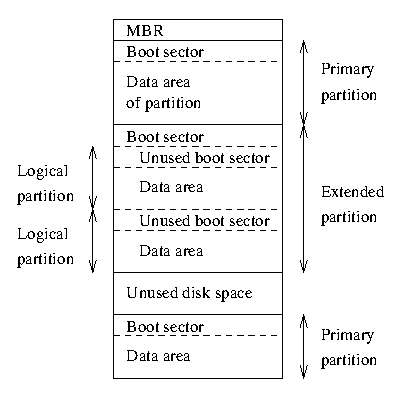
\includegraphics{disks/hd-layout.ps}
		%\include{hd-layout}
		\end{center}
		\caption{������ ���Ħ�� �����.}
		\label{fig:hard-disk-layout}
		\end{figure}

\subsection{���� ���Ħ̦� �����}

	�����æ ���Ħ̦� ����� ��� �������������Φ ������� (���� � ���� �
	MBR, � ��ۦ ����������� �� ���������� ���Ħ���) ����� �� �����
	����� (����� - ���� ���� �� ����� �������� ���Ħ� - �� ��
	��������, �� �� ��Ǧ����), � ����� �����դ���� ���
	צ���צ����� ���Ħ��. �� �������� ��� ����, ��� ����� ����
	��������� ��� �����æ��ϧ �������, �˦� �������� ����� ���Ħ�,
	��� ����������� ������ ���Ħ��. ���� ����� - ����¦���
	��������, ���� �צ Ҧ�Φ �����æ�Φ ������� ������ ���������
	�������������� ����� � ��� �� ���Ħ���.  �����, �������Ħ,
	�����æ�Φ ������� �� ���� �� ��������Φ Ҧ����� �������
	���Ħ̦�. ���������, ����� �� ������� �� ��� ���� ����ϧ
	�����. �� �� Ǧ��� - ���˦ � �����æ���� ������ ������������
	��� ������ ��צ���. ���������, �� ͦΦ��� ���˦ ���Ӧ�
	DR-DOS'� ��������� ���������� ¦� ������ �����, � ��� ���, ��
	��ۦ - צ��������� �� ����� � �������.

	����� �����������æ��� ������æ� �� ���� �������, ��� ��������
	����� צ���צ��� ����, ��� ���˦ ���¦��� �����Φ ��������
	�������Φ � �����æ~\ref{tab:partition-ids}. �� � ���� �������
	������� � �����Ħ \cmd{fdisk} ������.

\begin{table}[ht]
\caption{���� ���Ħ̦� ������� ���˦� (� �������� \cmd{fdisk} ������).}
\begin{center}
\begin{tabular}{rl rl rl rl}
\hline
0 & Empty               & 40 & Venix 80286  & 94 & Amoeba BBT     \\
1 & DOS 12-bit FAT      & 51 & Novell?      & a5 & BSD/386        \\
2 & XENIX root          & 52 & Microport    & b7 & BSDI fs        \\
3 & XENIX usr           & 63 & GNU HURD     & b8 & BSDI swap      \\
4 & DOS 16-bit $<$32M   & 64 & Novell       & c7 & Syrinx         \\
5 & Extended            & 75 & PC/IX        & db & CP/M           \\
6 & DOS 16-bit $\ge$32M & 80 & Old MINIX    & e1 & DOS access     \\
7 & OS/2 HPFS           & 81 & Linux/MINIX  & e3 & DOS R/O        \\
8 & AIX                 & 82 & Linux swap   & f2 & DOS secondary  \\
9 & AIX bootable        & 83 & Linux native & ff & BBT            \\
a & OS/2 Boot Manag     & 93 & Amoeba       &    &                \\
\hline
\end{tabular}
\end{center}
\label{tab:partition-ids}
\end{table}

\subsection{���Ħ����� ��������� ����� �� ���Ħ��}

	���դ ������ ������� ��� ��������� �� ��������
	���Ħ̦�. ���ۦ��� �����æ���� ������ ����� ��ϧ ����Φ
	��Ҧ���� ����� �������, � ����, �����̦ ������, ����Ѥ����
	��æ����� ������������� � ���Φ� �����æ�Φ� �����ͦ ��
	������� ��������� ��� ��������� ���Ħ̦� æ�� �����æ��ϧ
	�������, �� ��� �������, ���� ���� �������� ������ ���� �����
	�� �� ���������������, ��� ����, ���� ��ۦ ������ ��
	�ͦ���. ������ ��Ҧ��Ԧ� ����� ������� ����������� \cmd{fdisk}
	, ��������� � �����\begin{intnote}��������, �� �� צ���������
	Ԧ���� �� `PC-��Ȧ����' �����æ���� ������. `������Φ' �Φ���
	(���� SunOS, Solaris) ����� ��������, �� �����������
	\cmd{format}. ������� צ�ͦ�Φ��� ͦ� ���� ����� � ����, ��
	\cmd{format} (���̦����� ���ݦ �����æ� �Φ�Ӧ�) ����ͦ�
	�������, ��Ħ, ���� ���� ��������� �� � ���צ�����, � �
	������� (�� STDIN), ����� ������� �����צ��� ��������������
	������ �������� ����� �� ���Ħ��, �� ����������� ������� �
	�������� �� ����������� ����, ���� ���Ҧ��� �������
	(`���������') ����'����Φ ������� ������������ ��
	����������æ�. �����צ��� ������������ �����Ӧ� ������ ���� �
	���� ���¦����� ��������� �Φ��� ��� ������ �����������������
	���������.\end{intnote}. �������æ ������������ \cmd{fdisk} ������Φ �
	���Ҧ�æ Ц������ ��� �ŧ. ������� \cmd{cfdisk} ��Ħ��� ��
	����æ��� �� \cmd{fdisk}, ��� ��� ������ ������ �� ����Φ
	(������������� ���������).

	��� ����������Φ IDE ���˦� ��������� ���Ħ� (����� ���Ħ�, ��
	����� ͦ������� ���� �����æ��ϧ �������) ������� ������
	���Φ��� � ����� ������ 1024 ��̦��Ҧ� �����. �� �����������
	����� ��, �� ��� ����Ԧ ������� ���� ����������դ���� �����
	BIOS (�� ����, �� ������� ���������� � ���������
	�����\begin{intnote}����� � ���� - ������ `������� ���������' PC
	���'�������� � DOS��. ������� �Ӧ� �������� � 640 �����
	���������ϧ ���'�Ԧ - �� ���� �� ������Ħ� ��������. ����
	����� ��, �� PC ������ � ������������ ����ͦ (standard mode)
	Ц� ��� ������������, ������� ����Ȧ�Φ��� ������������ ����
	������ ��������� \cmd{gzip} - ���� �� ��ͦ������� ���Φ��� �
	���ۦ 640����� ���'�Ԧ. � �� ��� - �� ������צ��� Ԧ����
	PC-������, Φ ��ۦ ������, Φ ��ۦ �Φ��� �� ����� �������
	������������ ����.\end{intnote}), � BIOS �� ���� ��� ��, �� ������ �
	¦����, Φ� 1024-�� ��̦������. ������ ������� �������������
	��������� ���Ħ���, ���� �� ���� ������ � ����� 1024
	��̦��Ҧ�. ��� �� ������ Ԧ���� �� ��� Ц�, ���� �Ӧ �����,
	�˦ ����� BIOS, ����������� � �������� �����. � ��˦���� �
	��������� ���������� �������� ������������� ���̦� �� �����,
	�� ����Ѥ���� \emph{��������� ������� ��Ť�} �������������
	����� ���Ħ���. �� Φ���� �� ������� ������� �������, ��
	������������� ��� ����'���� ��� ���������� ���� �� ���
	�����������æ� �����. ���� ������ �������� ������Φ �
	���������� ��� ��������� ���Ħ� ���, ��� צ� צ� ������� ��
	˦��� ����� �� ������ 1024 ��̦����� \begin{intnote}������� � ������
	������� �������, ���� �� ������� ���� �������� ��� ����Ԧ �
	DOS ��� � ���� ��Ȧ����� - Windows'���. ������ �� � ���ݦ�
	����Φ��æ� Windows, � ������� - � ���ͦ���Φ���� Ц���Ħ ��
	������� ������ �������. ���� �� ����-������ � DOS'�
	������������� �������� \cmd{sys} (��� ���������� �����
	�����æ��ϧ ������� � ���������� ����� �� ����� ����,
	��������� �� ������� - ������ ��� ���� ��������� ���
	���������), �� ������� ��ͦ����, �� �� � �Ӧ� �������� ����
	����������� �������. ���� ������� ���� Ԧ����, ��
	צ������������, �� ������� ������������ �������, � ���� �� ��
	����� ������� �������� �� �ŧ ���� � ���� ����, �� �������
	\cmd{sys} צ��������� ������������� �������. �� צ����������
	����, �� DOS ���������� ������Φ ����� Ԧ���� � ������
	�������� ����� � �� ���� ��������� ���� ������� (� DOS'� ��
	��� ��������� �����, �� ������ ������ � ���Φ ����� C: -
	MSDOS.SYS ��� PCDOS.SYS ������� צ� ���������
	������� (���� �� � ����, �˦ ���'������, �� DOS
	�������� ������ �� Ԧ���� ����������, � �� ������ � ����̦
	���� DOS ��� ���Ʀ�� "<MS">) �� IO.SYS), ���� �� ����
	����������� � ������ ͦ�æ �����.

	����������� ������ ����� � � ��, ��: � ������ ���� �������
	������ ����������� ����������� � ����� 1024 ������ ��̦��Ҧ�,
	� � ������ - ����������� ���� ����� ������� ��������� Ԧ����
	������ צ������������� ���� (��, �������, �� �Ӧ� ��
	�����). �Ҧ� ����, �� �� Ǧ���, ������� ��������� ��������
	(����� �������� �� ����) ��������� ��ͦ��� ������� ���� ����
	�� ����. � �Ҧ��� ��� ��, ��� ���� �� ����� ��� ���� (�������
	�� ��� ��� Ҧ���� ���Ħ�� � Ҧ����� ��������� �� ���, � ����
	��� ���� ���Ħ� � ˦������ ������, �˦ ����� ���������� ��
	��������). 
	
	� ����-������ �Φ�Ӧ, ( ����� �� � �����������), �������
	������� ��� ���� ���� �� ������ ����������. ��� ��˦����
	������ Ħ������� � �������� ���������, �����ަ � �צԦ PC,
	���������� ����� ���������, ��� �� �¦��� - � ������ ���� ����
	�� ������ ��̦����� � ���� ������ ���������.\end{intnote}.

	���˦ ��צۦ ���Ӧ� BIOS'�� � IDE �������, ��������, �ͦ���
	���������� � �������, �� ����� ¦���� Φ� 1024 ��̦����. ����
	�� ����� ���� �������, �� ������ ������ ��� ��, �� Ԧ���� ��
	���������, ��� ���� �� �� ������Φ, �� �����Ħ�� ���� � ���ۦ
	1024 ��̦����.\intnote{��� ����� ������ � �� �����. ��̦ ����
	����� ��� ��, �� �������� ������� ������� ������ ����� ����
	�������� - ����� �� Φ� ���������� ͦΦ��� �������Ҧ�
	����Ȧ���� ��� ������������ �������. ��� ��������� ���צ�
	�צ�����, �� ����� ����ͦ������� ������� ���� �������ϧ
	������ϧ ������� - �� �������� 50����� (� � ¦�����Ԧ �����˦�
	��������� 15-20�����). �����, ����� ���Ħ� ��������� ����� �
	�� ����-����� ��������� ����� (�� ����������� ��̦������),
	��ͦ����� ��� ���Ħ� ������ ��������� ��� ����, ��� ����
	������, �� צ� ���Φ��� ������ � ���Ҧ���� �����. �� ������ ��
	������ æ�� �������� �� ���դ �����̦, ��˦���� ��˦ �����
	����� ����� �����, Φ� 1024 ��̦����. �����æ� �����
	��Ǧ��դ����, ���� ��� ����� ������� �� � Windows � �����
	�����, ��� �� ��� ���� �������.}

	����� ���Ħ� ������� ���� ����� ����� �����Ҧ�, ��˦����
	������� ������� ������ ������դ���� ������ ���ͦ��� 1~�����,
	����� ����� ���������. ������� ˦��˦��� �����Ҧ� �� �������
	��� Φ���� ������ݦ� �Ҧ� ���� Ԧ����, �� �����Φ� ������ ��
	���� �����������������, � ���˦ � ���Ӧ� \cmd{fdisk}
	���������� ��� ��� �� (�� � �Ҧ� ���� - �� ������ �����������).

	���� ��� ���Ҧ��� �ͦ���� ���ͦ� ���Ħ�� �����, �������
	��������� �� ����� ������ �������� - �������� �������� ���
	������, �� � �� ����� ���Ħ̦ (��� ������ �����, �� ��������
	��Ħ�Φ��), ������ ��� ���Ħ�, ��������� ����� � ��������� ��
	����� ���Ħ̦ ��� � �������ϧ ��Ц�. ���� ���ͦ� ���Ħ��
	�¦���դ����, ������� ��� ���Ҧ��� ���� ����� צ�����������
	(�� ���������� ��������� ��Ц� � צ����������) ���ͦ��
	��Ӧ�Φ� ���Ħ̦� �����.

	� ��˦���� ����� ������ ������ ��̦����, ������ ����������
	צ�Φ ���ͦ�� ���Ħ̦� ����� � ������� ����, ��� � ��������
	��������� ��� �������� � �����̦����� ��������� ���������
	��Ц� � צ���������. ���� �� Ԧ���� ������������ ������� �
	��Ӧ��, �˦ �� ���� � �� ��������� ����ϧ �ͦ�� (��,
	���������, �������-�����), �� ����� �����צ��� �����
	���������� � Ҧ�����Φ����� ���Ʀ����æ��� ��� �����. �� �����
	Φ���� ������� ����� � ��צ� �����ͦ, ����Ԧ�� �ͦ������
	���Ħ�� �� ˦���� ��ڦ�.

	��� DOS'� ���դ �������� \cmd{fips}, ��� ����������դ���� �
	�������, �� ��������� ��ϧ ����� �ͦ������ ���ͦ�� ���Ħ̦�
	DOS'� ��� ������������ �� צ��������� �����, ��� ��� �����
	������ �� ��� �� ����Ȧ��� ������.

\subsection{���æ���Φ ����� ������ϧ� �� ���Ħ�� �����}

	����� ���Ħ� � ����� ���������� ���Ħ� ��� �צ� �������
	�������� ����
	��������. �� �������Φ��� ����� ��� ���̦� �����������
	��ɤ������� ������ ���Ħ�� ����� Ц��� ����� ����� ������
	�����. �� �������Φ��� ����� ���ۦ ������ ���Ħ�� (� ��������
	1--4) � ��������� ���Ħ����, ��������� צ� �� ˦�����Ԧ, �
	������ 5--8 �����������Φ �� ��Ǧ����� ���Ħ����, ���������
	צ� ����, �˦���� ������� �������� ���Ħ̦� �� ����� � צ�
	����, �� ����� � �������� ���Ħ̦� æ ��Ǧ�Φ ���Ħ��
	�����������. ���������, \fn{/dev/hda1} - �� ������ ��������
	���Ħ� �� ������� IDE �����, � \fn{/dev/sdb7} - ���Ԧ�
	���������� ���Ħ� �� ������� SCSI �����. ������ ������ ���̦�
	������ϧ� ��������� �~\cite{device-list}.

\section{�����צ �������}
\label{sec:filesystems}

\subsection{�� ���� �����צ �������?}

	\defin{������� �������} - �� ����� �� ��������� �����, �˦
	���������������� �������� �������� ��� ����������
	�������æ� ��� ����� �� ����� �� ���Ħ̦ �����. �����, ������
	�������, - �� ����� ����Φ��æ� ���������� ���̦� �� �����. ���ͦ�
	����� ����� ���������� �� ����Φ� �� �̦� "<����"> ���
	"<�������� ���Ħ�">, ���� ���� ��� ��� ����� ���������Φ ��
	������ ����� �� ���Ħ̦. ����, ���� �� ���դ�� "<� ��� �צ
	�����צ �������">, ������, �� ��� ����� ������� �� ���ڦ, ���
	Ц����Ħ��, �˦ ������� ��� ������ ���̦�, ��� � ������� �
	������� - �� ��� Ц����Ħ�� �� ��������� ��������� ���� ext2
	("<��������� ������� �������">, �� �� ��������� �
	����Ӧ). ���ͦ����Ԧ ͦ� ������ �� ���Ħ��� �� ����� ��
	�������� ��������, ��� �� ����� �������� ���Ԥצ. ���� ���˦
	�������� (��������� ���� Ԧ, �˦ ��������� �����צ �������)
	������ ��������� ������������� � ���������\intnote{�
	���̦���˦� ��צ ����� � ��������� "<������"> � ������ �������
	���������� ���������� "<raw">(raw disk, raw sector, raw
	partition), ���� ���̦��� ��� �� ������������� �� "<�����">
	��� "<��������������">. �� ���ͦ���ϭ�� צ���������,
	���������, �� ��������� Ц����Ħ�� ��� �������ϧ �� �����
	������ϧ �������, ��� ������ �� ���æ������� ����� ���������
	Ц����Ħ�� �� ������ �����. �� ��������Φ��� �� �����
	����������դ���� "<cooked"> - ����� ���Ħ� �� ��������
	�������� �� �����. (����ϭ���� - cooked device,
	cooked partition, ����) - ����� "<������������"> (��������,
	Ц���������). ���̦���� �������� ����������� Ц��� �����
	�������� �� ������ "<æ�����">, ��� �� ͦ� ������ - ��
	�������. ���� �, ���Ħ������� �� ������� ��������������� Ҧ����
	������������ ������, ������ ������� � ����� ��������
	����������. ���� צ����, �� ����� ��� ���� ���������, �� ���
	���� ��� ���� � �� ��� ������.} �� ����� ��� ����
	���Ħ̦. ���� �� ����� ����� ��� ���Ħ̦ ��� ���դ �������
	�������, ���� ���� ������ ���������� ���� ������� ��� ��������
	����������. ���ۦ��� ������� ��������, �� צ�ͦ�� צ� ��������
	˦�����, � ��������� ��������� �, ����, �� ������� ��������� �
	���Ħ����, �˦ �� ����� ������ϧ ������� �� ��� (���, ��
	��������� �� � ����, - ����� ������� ������� �� ���� ����, ��
	���Ҧ���). 

	����� ���, �� ��������������� ���� ��� ���Ħ� �� �������
	�������, ���� ����� �Φæ�̦������. ��� ����� �� ����
	�����դ���� ����� �������æ� ��� Ц��������� ������ϧ �������
	� צ�������� �������. ��� ������ צ����� �� \defin{���������
	������ϧ �������}.

	���ۦ��� �������� ������ �Φ�Ӧ� ����� ���� ����� ��������
	���������, ��� ���-���� ����������� � ����������. �����Φ
	������� ��������� \defin{���������}\intnote{superblock},
	\defin{inode}\ref{dict:inode}, \defin{���� �����}\intnote{data
	block}, \defin{���� �������Ҧ�}\intnote{directory block} ��
	\defin{���� ������}\ref{dict:indirection}. ��������� ͦ�����
	�������æ� ��� ������� ������� � æ����, ����, ���������, ��
	�� ���ͦ� (�������� �������æ�, ��� ��� ���� � �����������,
	�������� צ� ����������� ���� ������ϧ �������). � inode
	���Ҧ������� ��� �������æ� ��� ������� ����, �Ҧ� ���� �����
	\begin{intnote} 
%
%
	����� ���� ��� inode, ��� �� ����� ���� ��� �צ� \emph{�������}
	inode. ������, ��� ������� ���ͦ��� ����� Ц���������, �� ����
	inode � � ������, � �� �����, �� ������ ����������, �
	������-�������� ���������, ��� ���������� �� inode. ���� inode
	��� ˦���� ��������, �� ������, �� ͦ� ������� ���������Φ
	"<�����˦ ������"> - hard link. ����� �צ Ҧ�Φ ��������
	������ ��������� �� ���� � ��� �� ���� - ��� ����������� ��
	�������� ���, Φ�� �� ���� ���� ��� ˦���� ����.

	�̦� ����� צ������� Ҧ����� ͦ� ��������� �� �'�����
	(�����̦�����) �������� (soft link ��� symbolic link,
	symlink). ���� ������� ������ �� �� �� ����, �� ������ ����
	����� ������ � ���� � �����, �� �����̦��� ������ - ��
	���æ������ ��� �����. ���� ���������� �� �����̦��� ������,
	���������, �������� \cmd{ls -l}, �� ��ͦ���, �� �����̦���
	������ - �� ���� ���� ���������� ���ͦ��, ����� 10-14 ����. ��
	� ���� æ �����? �� - ������ ������� �� ���Ǧ���� (�� ������
	"<������">) æ�� �����̦��ϧ ������. 

	���, ���������, ���� �����̦��� ������ ���� �������� �����
	��������, �� \cmd{ln -s /usr/X11R6 /usr/X11 }, �� ����
	\fn{/usr/X11} ���� �����̦���� ������� �� \fn{/usr/X11R6}, �
	���� ���ͦ� ���� Ҧ��� 10 ���� - ����� ˦��˦��� �����̦� �
	\texttt{/usr/X11R6}, ����� �� '/'.

\verb|#| {\sl ln -s /usr/X11R6 /usr/X11} \\
\verb|#|ls -l \\
\verb|#|total 42\\
\verb|#|lrwxrwxrwx   1 root     root           10 Mar 31 08:22 X11 -> /usr/X11R6/\\
\verb|#| [...]\\

	��� ��������� ���̦� (� ���� ���̦ � צ� �������� ������)
	�����̦�Φ ������ צ�Ҧ�������� ������ �������� � �����, ��
	����դ ��� ����� - ����� � ���� ���Ԧ inode, �� �����դ����
	��� �����, � �����̦��ϧ ������ �������� "<l">.

	\end{intnote}.  ����� ����� �����դ���� � �������Ҧ� ����� � �������
	inode'�. inode ���Ҧ��� ������ ˦����� ���˦�, � ����
	��������� ��� ����. ��� � inode'� ��������� ͦ��� Ԧ���� ���
	˦����� ���˦� �����, �����, ���� ���Ҧ��� ���� ¦����, ���
	������ �� ������Φ ����� ����ͦ��� ��Ħ�Ѥ���� ¦����
	ͦ���. � �����, �� ��Ħ������� ����ͦ���, � ���������
	�������. �����, ���� �� ����� ����դ �� ��, �� ����, Φ�
	��������� ��Φ � �����, ���Ҧ��� ������, �� ����������� ���
	����, ������������ ������� �� �����.

%	\meta this needs rewriting.  
	�� �������� �����צ ������� �Φ�Ӧ� ���������� ���� ����� �
	\defin{"<Ħ�����">} (�� �������� �� ��������� �������
	\cmd{lseek}, ����� Ħ������� ��� ��� ����� � ���Ҧ���
	Ц������). ���� � ���̦ �������, �� ������� ������� ������
	������ ������, Φ���� ����� ����� ͦ��� � ���̦ ��� ���ͦ�
	���� ���Ԧ�, ��� ������� ��������� �������� ��� ����� ��
	������դ���� �� �� � ������ ���̦ (����� ���� �������Ħ ����
	��������������� ����� ����� ��������� ��������). ��
	�����Ѥ���� �������� ����� ��� ��������� �צ������ ���̦�,
	¦�̦���� ��� �Ц������ ������������ � ����Ӧ, ������ ���
	����� �� ������ ���æ������ �����˦�. (���� �����������
	������������ ����ϧ ���æ����ϧ �������� � ���æ ������ ���
	� inode'�. �� ������� ������ �������, �� ��� ����� ����� ��
	צ��������� �������� �� �����, ����� � ���̦ - Ħ���.)

	���� ������ �����Φ. �� �����ͦ ������ ������ ��ͦ�������
	��������, �� Ħ��� ���Ҧ����� ������� 4~����� � 200~�����
	�����. �������� ������� ��� צ������ ���� ������� � �� ��� ���
	�����. ��Ӧ� ��� ��ͦ������� Ħ��� �������� �
	�������~\ref{chap:measure-holes}. \begin{intnote}
%
	����Φ��� Ħ��� � ������ ������ ���� ���������� ���˦
	����ɤ���ݦ. ���� ����� ���'����� ��� �� � ���� ������ Ħ���
	������ ���������� � �� ����� ������, ��� æ Ħ���
	"<��������">.

	���, ���������, ����� � ���¦��� �����������Φ��� ��Ц�
	���̦�, � ���� ������ ���������� Ħ��� � ����� ��� �����
	dbm. ��˦ ����� ���������������� � ����� ����� ���
	NIS~\ref{dict:nis} ��� � ����� ����� ���������ަ�, �˦
	���������������� � \cmd{sendmail} ���Ӧ� 8.x. 

	����� ��, ������ �����Ѥ����, �� ���� ���ͦҦ� �Ӧ� ���̦� ���
	����� ���� ���� ¦�����, Φ� ���ͦ� ��������� ���Ħ��, ����
	ͦ����� ��˦ �����. ���� � ����֦ ������� ˦���� �����Ҧ� NIS,
	�� ���� ������Ԧ�� ��������� �� ��������� - ���� ��������
	������ (master) � �Ӧ ��ۦ �������-Ц����̦ (slave). ���
	����Ȧ����Ԧ �������� ���� ����� �� Ц������� ��������
	����������դ���� ������� \cmd{xfer}, ��� �������� ������
	��Ц������ ���̦� ��� ����� � ��������� ������� �� Ц����̦.
	�� � ���� ���� � ������Ц ������ ������� \cmd{rcp}, � ����
	����� �� ����� Ħ���, �� Ħ� ���� ������ ���������. ���
	������� \cmd{rcp} "<�� ����ͦ�"> Ħ��� � � ������� ���̦� �
	Ħ����� ������������ ������� \cmd{rcp} ��������� �� ����, ��
	��Ц� �����Ѥ���� ¦����� ��ɭ����� � �������� ���Ħ�
	�������� ������� ���� ������������� � ��� ���, �� ��
	��������� �����Ҧ �� ���� ����� צ������ ͦ���.  \end{intnote}

\subsection{����� �� �������x �������x}

	����� Ц�����դ ˦���� �������� ������, ����� ����
	��������צ���� �:
		%
	\begin{description}
	\item[minix]

		������Ҧ�� � �Ӧ� � ���������� ���¦���
		������������� �� ��צ��. � ��� �� ���, ���� ������
		�������� �� ������������ (צ����Φ ���˦ ����צ
		צ������\intnote{time stamps}, ������� ����� �����
		�������� 30-�� ̦������ , ���� ���� �������� 64~������
		�� ������� �������).

	\item[xia]

		�����ͦ���� ���Ӧ� ������ϧ ������� minix, ���
		��������� ��֦ ������ ����� ����� �� ���ͦ� ������ϧ
		�������, ��� �� ������ ����� ����������� ��
		�������. �� - �� ���� ��������� ������� �������, ���,
		��  ��צ���������, ������ ������ �����. 

	\item[ext2]

		���¦��� ������ ������������ Ҧ��� ������� �������
		������, �� ����� ������ - ���¦��� �������, ����
		������������ ����� �����, ��� �� ����� ����� ����
		����������� �� ����������� ������ ������������, �����
		��צ ���Ӧ� ���� �������� ������ �� ������ ��������
		���������� �������� �������� ������.

	\item[ext]

		���Ҧ�� ���Ӧ� - ����������� \texttt{ext2}, ��� ����
		������������ ��� ����� ��� ����������. �� ���������
		��� ����� � ����� ��������, � Ԧ ��� ��� �� � ������,
		��� ��ͦ���� �� ����� ���Ӧ��.

	\end{description}
		%
	��������� �� �����, ���դ Ц������� ��� ������ "<���������">
	�������� ������, �� ������ ����Ԧ��� ��ͦ� ������� � ������
	���������. �Ӧ æ ������Φ ������� �������� ��������� ���
	����, �� � Ҧ�Φ �����צ ������� ������, ��� ������� ���� ��
	����� ��� �� ����� �����������, �˦ ������Φ � �Φ����, ���
	����� ���˦ �ͦ�Φ ��������� ��� �� ��.
		%
	\begin{description}
	\item[msdos]

		��ͦ�Φ��� � DOS (� ����� � OS/2 �� Windows NT) -
		�����צ ������� FAT. 

	\item[umsdos]
		���������� ������ϧ ������� \texttt{msdos} ��� ������
		- ��� �������� ������ ���� ���̦�, � �����צ���
		�����Ϥ��� ������˦� ������,
		�����̦�, ������ �� ���̦� ������ϧ�. �� ����������
		������Ѥ ������������� ��������� �������� ��������
		\texttt{msdos}, ��� �� ���� �� - ������� �������
		�����, � ����� ����� צ������ ����Ȧ�Φ���
		������������� �������� �������� ��� ������ ���
		�������Ԧ ����'����� � ������������ DOS'��.

	\item[iso9660] ���������� ������� ������� �������-���˦�, ���
		��������� ���������� "<��� ���">, ��� ������Ѥ
		������� ���Ǧ ����� ���̦�. ���������� ��� ��� ���
		����Ȧ����Ԧ Ц����������� �����������.

	\item[nfs]
		
		������� ������� ����֦ \intnote{networked file system
- NFS} - ������� �������, ��� ������Ѥ �Ц���� �� �������� ����'������
� ����֦ ������������� ������� � ������Ѥ ������� ������ �� ��� �
����-����� � ����'���Ҧ� ����֦.
			
	\item[hpfs]
		������� ������� OS/2.
	\item[sysv]
		�����צ ������� SystemV/386, Coherent �� Xenix.
	\end{description}
	\begin{intnote}�� ����� ����� ������ ���˦ �������צ ������� ��
		�����Φ � ��ɭ���̦.
		\begin{description}
		\item[vfat]
		������� ������� ������������� � Windows 95 -
		���������� ������ϧ ������� DOS, ��� ������Ѥ
		������������� ������� ������� ���̦�. 

		\item[hfs]

		"<�����Ȧ��� ������� �������"> (hierarchical
		file system), ��� ��������դ���� � �����æ�Φ� �����ͦ
		MacOS �� ��˦������. �� ������� ���� ���� ��˦ ���
		������������ - ��� ������� ������ ��������� ��
		��˦���ۦ, �� (� �Ϥ����Φ � ���̦��æ�� ���������
		Ҧ��ϧ ��˦���ۦ����ϧ ����֦ AppleTalk) ���
		�������� ���� ������� ��� ����֦ Mac'�� (�����
		������Ѥ, ���������, ���������� ��˦�����������
		�������-���� �� ������������ ���� ��� �Ӧ�� ����֦
		Mac'��).

		\item[ufs]
		������� �������, �� ��������դ���� � SunOS ��
		Solaris. � ���ͦ���ϭ�� SunOS - �� ������� �������
		���� "<4.2">, � � Solaris'� ���� � ������ �����
		"<ufs">. ���� ������� ������� ������� �������� ���
		Sparc Linux'�, ���̦���� ������Ѥ �Ц����
		������������� ��������� ��������� SunOS/Solaris �
		Sparc ������.
	\end{description}
	\end{intnote}
		%

	��¦� ������ϧ ������� �������� צ� �����æ�. ���� �� ������
	 ���� ������ �� ����� � ��� �� ���̦� � ������ �� � ��ϧ��
	 ���ϧ �����æ��ϧ ������� (����������ϧ �� ����� �
	 ����'���Ҧ), �� ������� ����������������� ������� �������
	 ���� æ�� �����æ��ϧ �������. ���� � �� ����� צ����� ��¦�,
	 ��Ħ ��������� ������� ���� ������� ������� ext2, ��˦����
	 ���� ��� �Ӧ ����Ȧ�Φ ����æ� � ��������� ������.

	�Ҧ� �������� ���� �������� ������ � ����Ӧ � ����� �������
	������� \texttt{proc}, ���������� � �������Ҧ� \fn{proc}, ���
	�������Ħ �� � �������� ��������, ���� � ���� �� �ŧ
	�����. ������� ������� \texttt{proc} ������դ ������ ��������
	����� �������Φ ���� � �����Ӧ� (�צ��� � �����). ���� �����
	�����������צ æ ��������� � �����Ħ ������ϧ �������, � ��
	����� � ������ �����Ħ ����� ������������� ������Φ ������ ���
	������ � �������. ���������, ��� ����, ��� �������� ������
	�Ӧ� �����Ӧ� � �����ͦ ����� �������������� ��������

	%
	\begin{quote}\tt
\verb|$| {\sl ls -l /proc} \\
\verb|total 0| \\
\verb|dr-xr-xr-x   4 root     root            0 Jan 31 20:37 1| \\
\verb|dr-xr-xr-x   4 liw      users           0 Jan 31 20:37 63| \\
\verb|dr-xr-xr-x   4 liw      users           0 Jan 31 20:37 94| \\
\verb|dr-xr-xr-x   4 liw      users           0 Jan 31 20:37 95| \\
\verb|dr-xr-xr-x   4 root     users           0 Jan 31 20:37 98| \\
\verb|dr-xr-xr-x   4 liw      users           0 Jan 31 20:37 99| \\
\verb|-r--r--r--   1 root     root            0 Jan 31 20:37 devices| \\
\verb|-r--r--r--   1 root     root            0 Jan 31 20:37 dma| \\
\verb|-r--r--r--   1 root     root            0 Jan 31 20:37 filesystems| \\
\verb|-r--r--r--   1 root     root            0 Jan 31 20:37 interrupts| \\
\verb|-r--------   1 root     root      8654848 Jan 31 20:37 kcore| \\
\verb|-r--r--r--   1 root     root            0 Jan 31 11:50 kmsg| \\
\verb|-r--r--r--   1 root     root            0 Jan 31 20:37 ksyms| \\
\verb|-r--r--r--   1 root     root            0 Jan 31 11:51 loadavg| \\
\verb|-r--r--r--   1 root     root            0 Jan 31 20:37 meminfo| \\
\verb|-r--r--r--   1 root     root            0 Jan 31 20:37 modules| \\
\verb|dr-xr-xr-x   2 root     root            0 Jan 31 20:37 net| \\
\verb|dr-xr-xr-x   4 root     root            0 Jan 31 20:37 self| \\
\verb|-r--r--r--   1 root     root            0 Jan 31 20:37 stat| \\
\verb|-r--r--r--   1 root     root            0 Jan 31 20:37 uptime| \\
\verb|-r--r--r--   1 root     root            0 Jan 31 20:37 version| \\
\verb|$|
		\rm\end{quote}
		%

	(�Ҧ� ��������� ��� ���� �� ˦���� ���������� ���̦�, �˦ ��
	����� צ���צ���� �����Ӧ�. �������, ��������� ���, �����
	���������� ��Ҧ����� � �������� �����æ��.)

	���� \texttt{/proc} � ����������� �������� ��������, ����� ��
	������� ��צ�� � �� ���������� �����. ���� ��� ���դ Ԧ����
	� ��צ ����. ���� ����-��� ����������� ���������� �� ����-��ϧ
	� ������ ������ϧ ������� \texttt{proc}, ���� ����� �� ���,
	Φ�� �� ���� �����Ħ ���դ ����. ����, ��צ�� ���� �� ��������
	����� ������ ��� ������-����������� ���� \fn{/proc/kcore}, צ�
	�� ������ ������� ����� ���'�Ԧ Φ �� �����, Φ � ���'�Ԧ (��
	���� ����, ���� �� �� ������� ���� ������� ����-������).

\subsection{���� �������� �������� �������������?}

	� ¦�����Ԧ �����˦� ����� ������� ����� � ����������Φ
	�������� ��������� ��������� ���������. ����� ���¦���
	���������� � ext2fs, �, ������� ����, ����� ������
	������������� ���.  � ��������Ԧ צ� ���������� ����� ��
	���������, �������Ԧ, ��Ħ����Ԧ, ��ͦ����Ԧ, ����, �̦�
	��������� ����� Ԧ �� ��ۦ ������� ���� ext2fs. ��� ˦�����
	��������� Ҧ����� ������ �������� צ� ���������� ����.

\subsection{��������� ������ϧ �������}\label{sec:mkfs}

	�����צ ������� ���������� (��� "<�Φæ�̦�������">) ��
	��������� ������� \cmd{mkfs}. �������Ħ �, ��� ����ϧ ������ϧ
	������� ���դ ���� ������ �������. ������� \cmd{mkfs}
	������-�������� ����� �� æ�ϧ ����� ������, � ��� ��������� �ϧ
	��� ���ϧ ������ϧ �������, ��������դ���� צ���צ��� ��
	�������. ��� ������ϧ �������, ��� ����� ��������, ��������� �� 
	��������� ��������� \texttt{-t ���\_������ϧ\_�������}
	�����Ħ \cmd{mkfs}.
	
	��������, �˦ ������������ �������� \cmd{mkfs}, ����� Ҧ�Φ
	���������. ������Φ (� ���¦��� �����צ) ��������� ������Φ
	�����, ��� �������Φۦ ��Φ ����� ������ צ������� � ���Ҧ�æ
	Ц������ �� �������Φ� �����Ħ.

	\begin{quote}
	\begin{description}
	\item[{\tt -t} {\it ���\_������ϧ\_�������}] ����Ҧ�� ���
	������ϧ �������.
	\item[{\tt -c}] ������ �¦�Φ ����� �� �������� �� ������.
	\item[{\tt -l} {\it �����\_�����}] ��������� �������� ������
	�¦���� ���˦� � �����  {\it �����\_�����}.
	\end{description}
	\end{quote}
	%
	��� �������� �� �����Ԧ ������� ������� ���� ext2, ���Ҧ���
	�������� ��˦ �������:
		%
		\begin{quote}\tt
\verb|$| {\sl fdformat -n /dev/fd0H1440 } \\
\verb|Double-sided, 80 tracks, 18 sec/track. Total capacity 1440 kB.| \\
\verb|Formatting ... done| \\
\verb|$| {\sl badblocks /dev/fd0H1440 1440 $>$ bad-blocks} \\
\verb|$| {\sl mkfs -t ext2 -l bad-blocks /dev/fd0H1440} \\
\verb|mke2fs 0.5a, 5-Apr-94 for EXT2 FS 0.5, 94/03/10| \\
\verb|360 inodes, 1440 blocks| \\
\verb|72 blocks (5.00%) reserved for the super user| \\
\verb|First data block=1| \\
\verb|Block size=1024 (log=0)| \\
\verb|Fragment size=1024 (log=0)| \\
\verb|1 block group| \\
\verb|8192 blocks per group, 8192 fragments per group| \\
\verb|360 inodes per group| \\
\verb||\\
\verb|Writing inode tables: done     | \\
\verb|Writing superblocks and filesystem accounting information: done| \\
\verb|$|
		\rm\end{quote}
		%

	������ ������� ������դ���� (�������� \texttt{-n} �������Ѥ
	����צ��� ������� �� �¦�Φ �����). ���� ����� �¦�Φ �����
	��������� �������� \cmd{badblocks}, ���������� ������ ��ϧ
	צ������������ � ����. �, �����Ԧ, ����������� �������
	�������, � ��� ����� ����������դ���� ������ �¦���� ���˦�,
	��������� �������� \cmd{badblocks}.

	��ͦ��� ������� \cmd{badblocks} ����� ��������������
	����������  {\tt -c}, ��� ����� צ������ ����Ȧ�Φ��� �
	����������� ���̦. ���� ������������ ������� �������� �
	���������� ������Ħ.
		%
		\begin{quote}\tt
\verb|$| {\sl mkfs -t ext2 -c /dev/fd0H1440} \\
\verb|mke2fs 0.5a, 5-Apr-94 for EXT2 FS 0.5, 94/03/10| \\
\verb|360 inodes, 1440 blocks| \\
\verb|72 blocks (5.00%) reserved for the super user| \\
\verb|First data block=1| \\
\verb|Block size=1024 (log=0)| \\
\verb|Fragment size=1024 (log=0)| \\
\verb|1 block group| \\
\verb|8192 blocks per group, 8192 fragments per group| \\
\verb|360 inodes per group| \\
\verb| | \\
\verb|Checking for bad blocks (read-only test): done| \\
\verb|Writing inode tables: done     | \\
\verb|Writing superblocks and filesystem accounting information: done| \\
\verb|$|
		\rm\end{quote}
		%
	���������� {\tt -c} ������ �������������, � ��������
	\cmd{badblocks} � ����������� ������, ��� ��� ����צ���
	������ϧ ������� Ц��� �� ��������� ����� ���-���� �������
	\cmd{badblocks}.
	
	������ ��������� ������ϧ ������� �� ��������� �����
	צ�Ҧ��Ѥ���� צ� ������� ��� ������ Ԧ���� ���, �� ���
	צ������ ���� ������������. 

\subsection{���������� �� �������������}\label{subsec:mount}

	����� ���, �� ������������� �������� ��������, �� �����
	\defin{����������}. ���� ����������, ��� ����, ���
	���������� � �������� �������, ������� �������� �� ����
	����'���� �� �������� ������ϧ �������. ��˦���� �Ӧ ����� �
	�Φ�Ӧ ���������Φ � ������� ����צ, Ц��� ����������
	�����Ѥ����, �� ���, �� ����������� �� ���������� � ����ͦ�
	�����צ� �����ͦ, ���� ��������� �������Ҧ�� � ����� ����צ.

	���������, �������~\ref{fig:hd-mount-root} �����դ ��� ����ͦ
	�����צ �������, ����� ڦ ��ϧ� ������� ������� (���������
	�������Ҧ��). ���� ����, �� �צ �����Φ �����צ �������
	��������Φ � ������ \fn{/home} �� \fn{/usr} ����ϧ ������ϧ
	�������, ����������� ����� ������ �������Ҧ� �������� ��
	�������~\ref{fig:hd-mount-all}.  

		\begin{figure}[thb]
		\begin{center}
		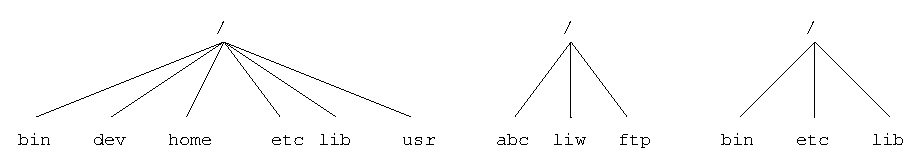
\includegraphics{disks/hd-mount-separate.ps}
		\end{center}
		\caption{��� ����ͦ �����צ �������.}
		\label{fig:hd-mount-root}
		\end{figure}

		\begin{figure}[thb]
		\begin{center}
		\includegraphics{disks/hd-mount-mounted.ps}
		\end{center}
		\caption{\fn{/home} �� \fn{/usr} ����������.}
		\label{fig:hd-mount-all}
		\end{figure}

	�����æ� ���������� ����������� ���������� ���������:
		%
		\begin{quote}\tt
\verb|$| {\sl mount /dev/hda2 /home} \\
\verb|$| {\sl mount /dev/hda3 /usr} \\
\verb|$| \\
\verb|$| \\
		\rm\end{quote}
		%

	�����Ħ \cmd{mount} ���Ҧ��� ������ ��� �ҭ������. ������ �
	��� - �� ���æ������ ���� ��������, ���� צ���צ��� ����� ��
	Ц����Ħ�� � �������� ��������. ������ - �������Ҧ�, � �˦�
	���Ҧ��� ���������� ���� ������� �������. ���� ����, ��
	�������� æ �צ �������, ���, �� ����������� � �����������
	������� ��������, ���� ��������� �� ����� �������Ҧ�
	\fn{/home} �� \fn{/usr}. ������, �� "<\fn{/dev/hda2}
	\defin{����������} �� \fn{/home}">, �, ����ϭ���� ���
	\fn{/usr}. ��� ����������, �� ����������� � Ԧ�, �� ��ۦ�
	�����צ� �����ͦ (Ц��� �� ����������), �̦� ��������, ��
	����������� � Ԧ� �������Ҧ�, �� �˦� �� ������� �������
	����������, ���, �� Φ��-�� �� - �������� �������Ҧ�.
	���ͦ���� Ҧ����� ͦ� ���æ������ ������ ��������
	(\fn{/dev/hda2} �� �������Ҧ��, �� ��� ���� ����������
	(\fn{/home}. ������ � ��� ��� ������ �� "<������"> ����� (���
	���Ħ��), � ��� ���, �� ����� - ����դ ������ �� "<�����ϧ">
	�������Ҧ� �� �����. �������Ҧ�, � �˦� ����������� ����������
	������ϧ �������, ��������� \defin{������ ����������}.

	�������, �� ��� צ�ͦ������, Ц����������� �����צ ������� ��������
	��Ц�. ������� \cmd{mount} ����������� ������� ��� ������ϧ �������,
	��� ���� ����դ. ��� �Ҧ� ����� ����� ����� �������������
	���������� {\tt -t \sl ���\_������ϧ\_�������}, ��� ���� �������
	���. ������ �� ����Ȧ���, �� �����, �� ���� ��������
	�������. ���������, ��� ���������� ������� ������� DOS ��
	�����Ԧ, ���Ҧ��� �������� �������:
		%
		\begin{quote}\tt
\verb|$| {\sl mount -t msdos /dev/fd0 /floppy} \\
\verb|$|
		\rm\end{quote}
		%

	��� �������Ҧ�, �� �����Φ ��ϧ ����դ���� ������� �������, ��
	�����������, ��� ���� ���� ������, ��� ����Ȧ���, ��� ����
	��������. �����, �Ӧ �����, �˦ �������� � æ� �������Ҧ� ��
	���������� ������ ������������ ��� ����, �� ������� �������
	����������. (���� �˦ �����, צ����Ԧ �� ��� ���������� ������
	���������� ����������, ��� ����, �� � ����� � ���
	�������Ҧ�, �˦ ����� �����˦ ������ �� ���� � ����� ������
	������ϧ �������, ������ ���� ���������� � ������������� ���
	����� ����.) ��� �� ���������� ����ϧ �����, � ������ �����
	����� ����� ����������� �� �������. ���������, ��צ�� ��¦, ��
	\fn{/tmp} �� \fn{/var/tmp} � ��������, �� \fn{/tmp} �
	�����̦���� ������� �� \fn{/var/tmp}. �� ��� ������ �������,
	���� ������� ������� \fn{/var} �� �� ����������, ���
	���������� ���̦� ����������դ���� �������Ҧ� \fn{/var/tmp},
	��� ����������� �� ������צ� �����צ� �����ͦ. ���� ����, ��
	\fn{/var} ����������, �������Ҧ� \fn{/var/tmp} � ������צ�
	�������Ҧ� �������� �����������, � ��ͦ��� �ŧ
	����������դ���� ���������� �� �� �����Φ �������
	�������. ���� �������Ҧ� \fn{/var/tmp} �� ��������, �� ���� �
	��������� ������������� ����������� ������� �� ����, ��
	���������� \fn{/var}.

	���� �� �� ���������� ���������� ���� � ������� �������, ���
	����դ��, �� ������ �������������� ���������� {\tt -r} ���
	����, ��� ���������� �� ������� ������� � ����ͦ \defin{Ԧ����
	�������}\intnote{readonly}. ��������� ��� ��������, ����
	�������� ����-��� ������ �������� ��-������ � ������� �������
	� ���� �� ���� �ͦ������ ��� �������\intnote{file access time}
	�� inode'�� ���̦� � ��Φ� �����צ� �����ͦ. ���������� �
	����ͦ "<Ԧ���� �������"> ����Ȧ��� ��� ��Ӧ��, �� �˦ �����
	����������, �����, ���������, �� �������-�����\begin{intnote}����
	������ � ������� ������ ���������� ������� � SunOS ��� �
	Solaris'� ���� �������� ����� ���������� ��ͦΦ�������� �
	���������. � ����Ӧ, ���� �� ����������� ����������
	�������-����, �� �������� ��������� {\tt -r}, �� \cmd{mount}
	Ԧ���� ������� �����������, ��� ���� ���-���� �����դ. ��� �
	SunOS �� Solaris'� �� ��-�����, ��������� ������������, �
	��-�����, �����Φ ������ ��������� ���������� ���-���� �
	������������� ����� ���������, �� ��� ����� ������� ������� ��
	�����դ����. ������� �� ����� �� ��, �� ����� ����� � ���-��
	�������� ������ צ�Ҧ�������� � Ҧ���� ��������
	(\texttt{iso9660} � ����Ӧ � \texttt{hsfs} � SunOS/Solaris),
	� �����ͦ��� ������������ צ� ������������ ˦������ �Φ�����
	צ�����.\end{intnote}.

	������� ����� ������ ��� צ�ͦ��� ���� �����������, � ����: ��
	�� ����դ���� "<���� �����"> ������� ������� - ��, ���
	����������� \defin{��������� �������� ��������}\intnote{root
	filesystem}, �� ���� ͦ����� �������� �������Ҧ�. �������� �,
	�� �����ͦ��� ������, �� ������� ������� �� ����� ����������
	�� �����Φ ���ϧ. �����צ�� � ����� ������� ���� ������ - ��
	�������� � �����.\footnote{��� �� ����� ��צ������ ���̦�����
	��Ȧ�Φ ������ ���� ��� ��Ӧ���� �� �������������
	����}\intnote{Kernel Hackers' Guide}. �������� ������� �������
	��Ҧ���� �������� �����Ѥ���� ����������� ��� ������� �������,
	� ����� ������ ������������� �� ��, �� ���� ���������� - ����
	��������� ���������� �������� ������� �������, ������� ������
	�� �������������. ����� �ϧ ������ϧ �������, ��� ��Ǧ���
	����դ���� �� ��������, ��� ���Ц������� ������������� � ����
	����, ��� �������������� �� ��������� LILO ��
	\cmd{rdev}\intnote{����� � צ������Φ ������������ �������ϧ
	������ϧ ������� � �������� ����˦���, Φ� ��˦ �������, ��
	SunOS �� Solaris. � צ������Φ ���������� ������ SunOS ��ϧ��
	�� ���������� Ҧ�Φ, ����� ���� ����˦��� ��������� Ҧ���
	����. ��Ҧ�� ������ ��� ���� �� ������� Ц����Ħ̦ ����� - ��
	����Ц������� ����� � ����. ���� ���� �� ���� ������ ��Ҧ�� ��
	������� ���Ħ̦, ������ ������ ��������� � ������� ���� ������
	��� �������������� ��Ҧ�� (�� � ����դ���� � ����-���Ħ�� ��
	�����, ���� ������ ��� ���� ������ ���Ħ��� - ���
	"<�����Ц�������"> � ����. �� צ�ͦ�� צ� ������, SunOS �� ����
	��������� ��� ����-�������� � �� ��������� ���Ҧ����� ���Ħ��,
	������ �� �������������). ����� � ��������Ԧ, ��������� ���
	��Ҧ��, ������� ������������� ���-���� � �����-����� �������
	����, ��� ���� ������������� ��� �� �����. � Solaris'� �����
	������� ���Ħ� �������ϧ �������, �������� ����� � ���̦
	\texttt{/etc/system}, ��� ������� �������������� ��Ҧ�� Ц�
	��� ������ ������� ������� Ԧ����, ���� �� ����� ��������������
	���� \texttt{/etc/system}.}.

	��� ����Ԧ ������� �������� ������� ������ ����դ���� ��������
	� ����ͦ "<Ԧ���� �������">. ��Φ�� �� ��������� �����Ԧ�
	������������ \cmd{fsck} ��� ����צ��� æ̦����Ԧ ������ϧ
	�������, � ��Ԧ� ������� �������
	\defin{���������դ����}\intnote{re-mount} � ����ͦ �������
	������. ������� ������� \cmd{fsck} �� ������� ������������ ��
	����������� �������� ��������, ��˦���� ����-�˦ �ͦ�� ��
	������ϧ �������, ��� ���� ���� �����դ����, {\em ���������}
	����˦ ��������. ���, ��˦���� �������� ������� � ������
	������� ���������� � �������� Ԧ���� �� �������, \cmd{fsck}
	���� ���������� ���Ҧ�Φ Ħ����� ��� �������, � �����æ�
	�������������� ������ �Ӧ ���Ҧ�Φ �ͦ�� � ���'�Ԧ �� ����.

	� �������� �������� ��� ����Ԧ ���Ҧ��� ��������� ����� ��ۦ
	�����צ ������� (�Ҧ� �������ϧ �� ����). �Ӧ ���� ����������
	� ���̦ \fn{/etc/fstab}\begin{intnote} ��� \fn{/etc/vfstab} �
	������� �� Solaris'��\end{intnote}. �������æ ��� ������ ����� � �
	���Ҧ�æ Ц������ \man{fstab}. ��, �� ��������� �������צ
	�����צ ������� ���������� �������� צ� �������� �����Ҧ�, �
	�� ���� ���Ʀ�������� ����� ������� ��������� ��ͦΦ�������
	���, �� �� ���Ҧ���. ���� ���Ħ� ��� ������ ������ �������
	���� ��˦�����, � ����� ����� ���� �� ���������.

	���� ������� ������� ¦���� �� ���Ҧ���, �� ����� ������������
	�������� \cmd{umount}\footnote{�������� � �� ������� ���� �
	���� ������� \cmd{unmount}, ��� ̦���� {\tt n} ͦ������ ������
	���� � ������Φ 70-� � ��� ¦���� �� �'��������. ����-�����,
	������� �� � Bell Labs, NJ, ���� �� �� ����-������
	��������.}. ��� \cmd{umount} ���Ҧ��� ���� �������� - ���
	����� ���������� ������ϧ �������, ��� �� ���æ������
	����. ���������, ��� ����������� �������Ҧ�, ��������Φ �
	������������ ������Ħ, ���Ҧ��� �������� �������:
		%
		\begin{quote}\tt
\verb|$| {\sl umount /dev/hda2 } \\
\verb|$| {\sl umount /usr} \\
\verb|$| 
\verb|$| 
		\rm\end{quote}
		%

	������ۦ צ�����Ԧ ��� ������� ��צ���� � ���Ҧ�æ Ц������ ��
	Φ�. �� ��������, �� ������ ���Ҧ��� �������������� ����������
	�������. {\em �� ��������� ������ ��� ������� � ���������!}
	����� ��������� ����� � ���'�Ԧ, ��Φ ������ �����Ħ
	������������ �� ���� ������ Ц�Φ�� � �� ����'������ ������Φ
	�� ����, ���� ���� �� �� ������������ \intnote{�����æ�
	������������� ������դ, �� ��Φ ����������� � ���� �� Ʀ���Φ
	��Ӧ�.}. ����, ���� �� ��������� ������� ������ - ���������
	�ͦ��� ��ͦ��� �����. ���� �� Ԧ���� ������ � �������, ��,
	������� ���� ��������� �� ���������, ���, ���� �������� ����
	(��צ�� ���������), ����������� ���� ���� ����������.

	��� ���������� �� ��������������� �������� ������ ���Ҧ���
	���� ���צ�ŧ �����-�����������, ����� Ԧ���� ����������
	\fn{root} ���� �� ������. �������� ����� � ��, ��, ����
	����-��� ���� ��������� �� ��������������, ���֦�� ������� ��
	����-�˦� �������Ҧ�, ��, � ����� ������� ���� � ���� ������
	��������, ���������, ����������� ���� ������������� �
	\cmd{/bin/sh}, ��� ���� ����� ������� ��������. �����,
	��������� ������������ ������ ����� ��������� �������, � ���
	����� ���դ ˦���� �����¦�:
		%
	\begin{itemize}

	\item ���� �����������צ ������ \fn{root}'�. �������� � ��
		���Ǧ��� Ҧ����� � ����� ���� �������, ��� �
		�������Ԧ��. ���� ��������դ � ��� ��������, ����
		����� ����Ȧ����Ԧ ����������� ��� �������, �����
		�������� �� �������� ������������ �������� ��
		Ц��������� �� ����֦.

	\item �������������� ��������� ���� \cmd{sudo} ��� ���������
		������������ ������������ ��������� \cmd{mount}. ��
		��� �� �� �������� Ҧ����� � ����� ���� �������, ���
		���-���� �� ��� ������������ ��������������� �������
		�� ������ \fn{root}'�\footnote{������� �������� ˦����
		������.}.

	\item ������������� ������������ ������� ����� �������
		\cmd{mtools}, ��� ���������� ������� DOS ���
		���������� �������� ������. ��� ����� - ���� ������ �����,
		���� ���, �� ���Ҧ���, �� ��Ц����� ����� � DOS�������
		������ � �����, ��� ��������� ��������� � �Ӧ� �����
		��������.

	\item ����������� ������ϧ �������Ħ� ����� � צ���צ�����
		����������� ��� ���������� � ���̦ \fn{/etc/fstab}.
	\end{itemize}
		%
	��� ���̦��æ� ���������� ��Ҧ���� ����� ������ ��
	\fn{/etc/fstab} ��������� ����� �����:
		%
		\begin{quote}\tt
/dev/fd0            /floppy      msdos   user,noauto      0     0
		\rm\end{quote}
		%

	��������� � ����� ��˦: �����Ҧ�, ���� ����� ����������,
	�������Ҧ�, � �˦� ���Ҧ��� ��������� ������� �������, ���
	������ϧ �������, ���������, ������� ��������� ��������� ��Ц�
	(����������դ���� �������� \cmd{dump}), �� ����� ������� ���
	\cmd{fsck} (��� �������� ������� ��� ����, ��� ����������
	�������, � ����� ������� \cmd{fsck} ������� ����צ���� �����צ
	������ ��� ����Ԧ �������. 0 �������, �� ����צ��� ��
	���Ҧ���).

	�������� \texttt{noauto} ����¦��� ���������� ���ϧ ������ϧ
	������� ��� ����Ԧ ������� (����� ������� \cmd{mount -a} ��
	�����դ �� ������� �������). �������� \texttt{user} ������Ѥ
	��������� �� ������� ������� ����-����� �����������צ, �, (�
	ͦ������� �������) �������Ѥ ��������� ����-���� ������� (��
	����������, ��� � � ������������ setuid) �� ������������
	����-���� ���æ������ ���̦� ������ϧ� �� ���������ϧ �����
	����� ������ϧ �������.\begin{intnote}���ͦ����Ԧ SunOS/Solaris �
	������ ������� ��������� � ����, �� �������� \texttt{user}
	צ����Φ� � ���� ��� ��������. ����� ���������� ��
	������������� �������� ������ ��������� \emph{ Ԧ����}
	���������� ��ͦΦ�������� - \fn{root}'�. ��� �Ҧ� ��������
	�����¦� � �� ���˦, �� ���� �� ���������� ����� ��̦ ��
	������, � �� �����Ѥ���� �� ��� �� ��������, ��צ��, ���� ��
	��ͦΦ���դ�� SunOS/Solaris.\end{intnote} ���� ����� ����� �������� � ����
	\fn{/etc/fstab}, �� ����-���� ���������� ���� ����������
	������� ��������� �������:
		%
		\begin{quote}\tt
\verb|$| {\sl mount /floppy} \\
\verb|$|
		\rm\end{quote}
		%
	������� ����� (�, �������� �, ���Ҧ���) ��������������
	צ���צ���� �������� \cmd{umount}.

	\begin{intnote}� ���˦ ������ ��� ��������Φ ������ϧ �������,
	������ϧ � \fn{/etc/fstab}. ���� ������� ��� ����� - �������
	\cmd{mount} \emph{�������} ���� Ԧ���� ���� �������� - ���
	��'� ��������� ����� ��������, ��� ����� ����������
	������ϧ �������. ������ ��� æ� ���צ \cmd{mount} ������� �
	\fn{/etc/fstab} ��� ����, ��� ������ ��� ��ۦ ����Ȧ�Φ
	���������. ���� ��� ��������Φ �� ������������� �����������
	������ ������� \cmd{mount ����\_���� �����\_����������}, ��
	������� �� ���� ��������� �� \fn{/etc/fstab}, � ��������������
	���������� ������� ������� �������������, �, ��˦���� �� - ��
	\texttt{root}, ������� �������: 
	% 
	\begin{quote}\tt
\verb|$| mount : only root can do that \\
\verb|$| 
	\rm\end{quote}
		%
\end{intnote}
	
	���� ��� ���Ҧ��� ����������� �����צ��� ���������� ˦�����
	��Ц� ������, �� �����Φ ����������� ����� � צ���צ�Φ �����
	���������� ��� �Ӧ� ��� � צ���צ�Φ ����� ��� ������� ���� �
	\fn{/etc/fstab}. ��������� ������ ���� Ҧ����� ��� ���
	�Ӧ�. ���������, ��� ���� ������ �� ���� �������� ������ -
	MS-DOS �� ext2 �� ��������, ��� ���Ҧ��� ���� ��˦ ����� �
	\fn{/etc/fstab}:

		%
		\begin{quote}
		\small
		\begin{verbatim}
/dev/fd0    /dosfloppy    msdos   user,noauto  0  0
/dev/fd0    /ext2floppy   ext2    user,noauto  0  0
		\end{verbatim}
		\end{quote}
		%

	��� �������� ������ MS-DOS (�� Ԧ���� �������, � �����̦ - �Ӧ
	� ���), ���� � ������ �������� ������ �������������
	\texttt{uid} �� \texttt{gid} �� ���������� \cmd{umask}, �˦ �
	���������� �����Φ � ���Ҧ�æ Ц������ \man{mount}. ���� �� ��
	����� ������Φ, �� ���������� ������ϧ ������� MS-DOS ��� (��
	ͦΦ���) ������ �� ������� ��� ����-����, �� �����̦-�� ��
	������. 
	
\subsection{����צ��� æ̦����Ԧ �������� ������ �� ���������
	\cmd{fsck}}

	�����צ ������� - ���� �����Φ ����Ҧ���, � ����, � �������
	���Ӧ, ���� �����Φ �� �������. �̦�Φ��� ������ϧ ������� ��
	����Φ��� � Φ� ������� ����� ����צ���� �� ��������� �������
	\cmd{fsck}. �����Ħ ����� �������, �� ���� ������� ����������
	�Ӧ ������Φ �������, �˦ ���� צ������, � �����������
	�����������, ���� ����������� ��˦ � ���, �˦ �� �����
	���������. �� �����, ¦�̦����� �����Φ ��� �������� ������
	��� צ��������Φ ������ �����, � �������� � ���� �����������
	������ Ҧ��� (��� �� �����̦ �� �����). ��ϧ � ��������
	�������� ������Ԧ�� ����������� ����� �����ϧ �
	���������������Φ, ��ϧ � "<��̦ڦ"> �� ����� �������
	�������Ҧ�, ��, ���������, �� �������� �� ��������� �������.

	���ۦ��� ������ ��������� \cmd{fsck} ���������� ��� ����Ԧ
	�������, ���, �� ¦��ۦ��� ������� ����������� (�, ��� ����,
	�������������) �� ����, �� ������� �������
	�����������������. ������������ ڦ������ϧ ������ϧ �������
	��������� �� ����, �� ������ ���� �� Ǧ����: ���� ���������
	����� ������ϧ ������� ڦ�����Φ, ������������ ��� ��������
	���� Ԧ���� ������� �� �� Ǧ�����, �� ������� �� �� ¦�����
	����� �����. ���, � ������ ����, ����� ����צ��� ������ϧ
	������� �� ������� �������� �������� �� ��������� \cmd{fsck}
	���� ������� ������ ������ ���. �, ����� ��, �� �������
	��������� Φ���� �� ����������� ��� ����������� �������Φ
	�������, ��� ����, ��� �� ���������� ��� ������ �������, �
	����Ӧ �������� �� ������ �����ݦ�. ������ ����: ���� ���դ
	���� \cmd{/etc/fastboot}, �� ����צ��� �������� ������ ��
	��������. ������ ����: ������� ������� ext2 ��� ��������
	������, ���� ����դ �� ��, �� ���� �� ������� �������
	צ���������� צ��� ��� ������������ ��������Φ. ������, ��
	������� ������� ���� ������������ "<������"> (���� ���������
	����դ �� ��) \cmd{e2fsck} (���Ӧ� \cmd{fsck} ���æ�̦������
	��� ����צ��� ������ϧ ������� ext2), ���� �� ����צ���� ��
	������� �������. ��� �����, ��������, �������� ����������, ��
	����� ������������� �� ��������� �����ͦ �������. �� ������
	������ � ���˦� (� ������ \fn{/etc/fastboot}) �� ��ۦ� �����ͦ
	�������� צ� ��������� �����Ԧ� �������, ��� ���� � ���������
	���������� ext2 ��������դ ������� ����, ���� �� ������դ����
	\cmd{e2fsck}. ��� ������� ������� ���������� ��� ���������, ��
	���Ҧ��� ���� ������� �� �������� ���������. (����̦ ��צ����
	� ���Ҧ�æ Ц������ \man{e2fsck}).

	����������� ����צ��� ��������դ Ԧ���� ��� ��� ������, �˦
	���������� ����������� ��� ����Ԧ �������. ��� ����צ��� �����
	�������� ������, ��, ���������, ������, ������������
	\cmd{fsck}, ���������� �� ������. \begin{intnote}������� \cmd{mount}
	� ����Ӧ ��� ������ ��������. ���� �� ������ ����դ�� �������
	�������, ��� �� ���� ����צ����, ������� ������� ������������
	��� �� � �����, �� ��������դ���� ������������ \cmd{e2fsck}
	��� ����צ���.\end{intnote}

	���� \cmd{fsck} ��� ����צ�æ �������Ѥ �� ������� �������,
	��� ���� �� ���� צ������������, �� ��� ���� ������ Ԧ����
	���� � ����: ��� �����˦ Ц������ ��� ������ �������� ������
	�����̦ � ������ ���� ���������, ��� ����� ��������
	���. ����� - ������� ������, � ������� �� ������ ������� ��
	��������� ���ڦ�, Ц�����ϧ ����� ����� �� Ц�������� ����� ��
	������ �� ����������� ����� ����¦� ����������� �������æ�. �
	��Ԧ� �� �����צ��� ��� �� ¦����, ��� ¦̦ ����� � ��צԦ ��
	���צĦ �� ����� ��Φ ����� �������. �������� ������� ��
	\intnote{Theodore T'so} \cmd{debugfs} ���� ��� ��������� ���
	�����.

	������������ \cmd{fsck} Ԧ���� �� ������������� ��������
	��������, Φ���� �� ����������� (�� ����������� �������ϧ
	������ϧ ������� ��� ����Ԧ, ��� ����դ��� ��� ����� Ԧ���� ��
	�������). ����� ��, �� \cmd{fsck} ������ � "<������">
	���Ħ���� �����, ���� ���� �ͦ������ �����צ ������� ���, ��
	������� ��� �� ��צ�� �� ������������. � ���� �����æ���
	������� ������, �� ����ɤ����Ԧ \emph{ ����������}.


\subsection{����צ��� ڦ�������� ���˦� �� ���������  \cmd{badblocks}}

	����צ��� �¦���� ���˦� ����� ���������� ��Ҧ������. �� �����
	������ �������� \cmd{badblocks}. ���� ����� ������ ���������
	�¦���� ���˦�. ��� ������ ��Ԧ� ����� �������� \cmd{fsck},
	��� ���� �������� æ ��Φ � ��������� ����� ������ϧ ������� �
	���, ��� �����æ��� ������� ����� � ���� ��Ԧ� ������������
	��� �������� �¦�Φ ����� ��� ����Ӧ �����. ��������� �������
	�����դ �� �� �������.

		%
		\begin{quote}\tt
\verb|$| {\sl badblocks /dev/fd0H1440 1440 $>$ bad-blocks } \\
\verb|$| {\sl fsck -t ext2 -l bad-blocks /dev/fd0H1440} \\
\verb|Parallelizing fsck version 0.5a (5-Apr-94)| \\
\verb|e2fsck 0.5a, 5-Apr-94 for EXT2 FS 0.5, 94/03/10| \\
\verb|Pass 1: Checking inodes, blocks, and sizes| \\
\verb|Pass 2: Checking directory structure| \\
\verb|Pass 3: Checking directory connectivity| \\
\verb|Pass 4: Check reference counts.| \\
\verb|Pass 5: Checking group summary information.| \\
\verb| | \\
\verb|/dev/fd0H1440: ***** FILE SYSTEM WAS MODIFIED *****| \\
\verb|/dev/fd0H1440: 11/360 files, 63/1440 blocks| \\
\verb|$|
		\rm\end{quote}
		%

	���� \cmd{badblocks} ��צ����Ѥ ��� ڦ�������� ����, ���� ���
	����������� Ц� ����, \cmd{e2fsck} �����դ ����ͦ����� ���
	���� � ���� ͦ���. ���� ���� ���� ���������� ��������, ����
	���������, �� ����, ڦ������� �����.

\subsection{�������� � ����������}

	�� ������ ������� �������� ���� �� ���� �� ����������
	���̦���Φ��� ���˦�. ��� ����, ���� �������� � ��������� ("<��
	����������"> ���̦���Φ��� ���˦�) ������, �� צ�
	\defin{��������������}. �� ���������� ��������������� �����
	���Ҧ��� ¦���� ���� ��˦���� �������/��������� �������
	������� ������� ��� ����� ¦���� ����ͦ����. ���� ����� ���� �
	��������� ���������æ�, ���� � ��������, �˦ ����� ������
	����� � "<�������� �������"> �� � �������� ��������.

	������� ������� ext2 ����������� ���������� ���������æ� ��
	ͦΦ��ͦ, ������������ �Ӧ ����� ����� �����, ��צ�� ���� ��
	�� ����� �������� � ���̦������ ��������. Ext2 ���������
	��������դ צ��Φ �����, �˦ ����������� �� ��Ӧ����� � ������
	������� �����. ����� ��� ext2 Ҧ��� ���� ����� ����Ȧ����
	����������� ��� ���������æ�. ���դ �������� ���
	�����������æ� ext2, ��צ����~\cite{ext2-defrag}. 

	���դ ������ ������� �����������æ� ��� MS-DOS, �˦
	����������� ����� ����-����, ��� ��������� ���������æ�
	���̦�. ��� ����� ������ �����������æ� ����� �������
	����������� ������� ������� æ����� �� ������Φ ��Ӧ� �
	צ�������� �� �����. ��������� �������ϧ ��Ц� �����
	�����������æ�� �����̦ �������� ���� ��� ����-��ϧ ���ϧ
	��������, ��˦���� ������ ���� ���� ��������� Ц� ��� ������
	��������. 


\subsection{��ۦ �������� ��� �Ӧ� �������� ������}

	������� ��ۦ ������ ������Φ �� ���� ������� ��� ����Ԧ �
	��������� ���������. \cmd{df} �����դ �˦���� צ������
	��������� �������� ���������� �� �����צ� �����ͦ (��������).
	\cmd{du} Ц������դ �˦���� ͦ��� �� ����� ������ �� �� ����
	�������Ҧ� �� �Ӧ �� �����. ����צ �������� �����
	��������������� � �������Φ �� ͦ���� �� �����.

	\cmd{sync} �����դ �Ӧ �� ������Φ ��Ӧ �����, �˦ �����������
	� ����Ҧ ����, �� ����
	(���. ���Ħ�~\ref{sec:buffer-cache}). ���� Ҧ��� �����������
	�����æ�, ���� �� ���Ҧ��� ������ ������ - ������-�����
	\cmd{update} �����դ �� �����������. �� ���� ����������� �
	��������Ʀ���� �����æ��, ���� \cmd{update} ��� ����
	������-��ͦ���� \cmd{bdflush} ������, ��� ��� ���Ҧ��� �������
	�������, � ����� ���� ������, ���� \cmd{update} ������� ����
	������. 

\subsection{��ۦ ������ ��� ������ϧ ������� ext2}

	��������� �� �������, �˦ ��������� (\cmd{mke2fs}) ��
	����צ����� æ̦�Φ��� (\cmd{e2fsck}) ������ϧ �������, � �����
	����� ������������� ��� �������������, ��� � ����� �� ���������
	צ� ���� ������ϧ ������� "<�������"> ��������, ������� ���˦
	��ۦ ��������צ ������ ��� ext2.

	\cmd{tune2fs} ������� ��� Ц������ �������Ҧ� ������ϧ
	�������. ���˦ � ���¦��� æ����� �������Ҧ� ��˦:

		% 
       \begin{itemize} 

       \item ���¦���� ��������� ˦��˦��� ���������. ���� �������
             ������� ���� ���������� � ������������ ��� ����צ���
             ������ ��ڦ�, \cmd{e2fsck} �������� ����צ�Ѥ �������
             �������, ��צ�� ���� ���� ���� ������������ �����. ���
             ������, �� ���������������� ��� �������� �� ��� 
             ��������������, �������� ������� ���� � ��� �����
             ��������.

        \item ������������ ��� ͦ� ����צ�����. \cmd{e2fsck} �����
                ���� ��������� ����צ���� ������� �������, ���� ���
                ͦ� ����צ����� ���������, ��צ�� ���� ���������
                ������� �����������, � ������� ����դ���� �� ����
                �����. �����, ��� �������� ����� צ�ͦ����.

        \item ���˦��� ���˦� �������������� ���
                \texttt{root}'�. Ext2 ������դ ����� ������� ���˦�
                ��� ������������ \texttt{root}'��. ����� �����,
                ��צ��, ���� ������� ������� ��������������, ���
                ���������� ��ͦΦ�������� ��������� ������ ����Ԧ�, �
                �� ����� ���� ������� �� �������� ���̦�. �� ������,
                ����� ��������� ����Ԧ� �������������� �� Ҧ�Φ 5\%,
                �� ��� ¦�����Ԧ ���˦� � ����������� ���������. ���
                ������, �����, �� ��� ����� ����� ������������
                ������� �����.

	\end{itemize}
		%
        ���Ҧ��� Ц������ �� \man{tune2fs} ������� ��� ¦����
       �������æ� �� ������ͦ.

	\cmd{dumpe2fs} �����դ �������æ� ��� ������� ������� ext2, �
	��������� �������æ� � �����-�����. ������ ����, �� ����� ��
	�������� �������� �� ���.~\ref{fig:dump2fs-output}. ���˦
	��Φ, �� ��������� � ������ ���Φ����� � ���������� ����ͦ���
	����, �� ������ ������� �������
	(���. �������~\ref{chap:ext2fspaper}, ��� ¦��ۦ��� �����ͦ��
	��צ�� ��������� ��ͦΦ���������. 


\begin{figure}[t]
\begin{center}
\small
\begin{verbatim}
dumpe2fs 0.5b, 11-Mar-95 for EXT2 FS 0.5a, 94/10/23
Filesystem magic number:  0xEF53
Filesystem state:         clean
Errors behavior:          Continue
Inode count:              360
Block count:              1440
Reserved block count:     72
Free blocks:              1133
Free inodes:              326
First block:              1
Block size:               1024
Fragment size:            1024
Blocks per group:         8192
Fragments per group:      8192
Inodes per group:         360
Last mount time:          Tue Aug  8 01:52:52 1995
Last write time:          Tue Aug  8 01:53:28 1995
Mount count:              3
Maximum mount count:      20
Last checked:             Tue Aug  8 01:06:31 1995
Check interval:           0
Reserved blocks uid:      0 (user root)
Reserved blocks gid:      0 (group root)

Group 0:
  Block bitmap at 3, Inode bitmap at 4, Inode table at 5
  1133 free blocks, 326 free inodes, 2 directories
  Free blocks: 307-1439
  Free inodes: 35-360
\end{verbatim}
\end{center}
\caption{������ ������  \cmd{dumpe2fs}}
\label{fig:dumpe2fs-output}
\end{figure}

	\cmd{debugfs} � צ��������� ������ϧ �������. ��� ������Ѥ
	������ ������ �� �������� �����, �� ����������� �� ����, �����
	���� ����� ��������������� ��� צ��������� ��� ���˦�, �˦
	ڦ�����Φ ���Ԧ����, �� \cmd{fsck} צ������� �� ��� ��
	����. ��� �� �������� ����� ������������� ��Φ, �� 
	\cmd{debugfs} ����� ��������������� ����� ��� צ���������
	������� ���̦�. �����, ������ � æ�� ��������� ������� ����
	�������� ����� ����, �� �� ������ �������. ��������Φ ������
	������ ������� �Ӧ ��ۦ ��Φ. 

	\cmd{dump} �� \cmd{restore} ������� ��� ��������� ���������
	��Ц� ������ϧ ������� ext2. ���� �������� �� �����æ����
	����¦� �Φ��� �� ��������� �������� ��Ц�, ��� � �����Ʀ�����
	��� ������ϧ ������� ext2. ������Φ�� �������æ� ��� �� � �
	���Ħ̦~\ref{chap:backups}.

\section{����� ��� �������� ������}

	�� �Ӧ ����� �� Ц����Ħ�� ���������������� �� �����צ
	�������. �����Ħ�, �� ͦ����� ����Ԧ� ��� ���Цέ�,
	���������, �� ��� ������ϧ �������. ���ۦ��� ������
	���������������� ��Ħ��� �� ��Ҧ���, ���, �� \cmd{tar} �� ��ۦ
	��Ħ�Φ �������� ��������� ��Φ ������������� �� ���� ���
	������ϧ �������. �������������Φ ������� ������ �� ����� ������ϧ
	�������, � ͦ����� Ԧ���� ���� �������.

	������� צ� ��������� ������ϧ ������� ��� Ԧ ��������, ��
	�������� ����Ԧ� ����������դ��� ¦��� ����� "--- ��� ����ϧ
	������ ���� �� ��̦��צ ����æ� ������ϧ �������. �Ҧ� �����
	��˦ ����� � ¦��� ��ͦ����� � ������ ���������. ���������,
	��� �Ӧ� ������ ������ \cmd{tar} � ����� � ��� ��, ��
	��������� �� ��, �� �����צ ������� צ�Ҧ�������� צ� ��Φ��
	������� �� ���ϧ. �� ������ �������� ������������� ������� ���
	�������� ������ � ��ڦ ����Ȧ����Ԧ. �������������Φ ����� ������
	��� ����� �� ����� ������ϧ �������, ���� ������ � ����.

	�� ���� �������� ��� ������������ "<������"> ������� �
	����Ȧ�Φ��� ������� ��Ц� "<������"> ��� ���������� �
	���. ���������, ���� �� ����� ����������� ������� �������, ���
	Ԧ���� �������� ����������, ����� � ������� ����� ��Ц�
	������ϧ �������, ����, Φ� ���������� �� צ�������, ��˦����
	� ��ڦ �����ަ �� ������ ������� ������ ��������. ���� ��
	�����¦� �� ������� - �� ��������� ������� \cmd{dd}:

		%
		\begin{quote}\tt
\verb|$| {\sl dd if=/dev/fd0H1440 of=floppy-image} \\
\verb|2880+0 records in| \\
\verb|2880+0 records out| \\
\verb|$| {\sl dd if=floppy-image of=/dev/fd0H1440 } \\
\verb|2880+0 records in| \\
\verb|2880+0 records out| \\
\verb|$|
\verb|$|
		\rm\end{quote}
		%

	����� ������� \cmd{dd}	������� ������ ����� ������� � ���̦
	\fn{floppy-image}, � ����� � ��� �����դ �� ���������� ��
	������� (���Ħ�������, �� ���������� ������������ ��ͦ����
	������� � �������Ħ ͦ� ����� ���� ���������. ������ �� ����
	������ ��� ���� �����.). 

\section{��Ħ����� ��������� ��������}

\subsection{����� ���Ħ�� ���˦�}

	���� ������� ������� ���� �� ���Ħ�� ��������� �����. � �� ��
	Ǧ��� - �� ���դ Φ��ϧ �Φ��������ϧ ������ �� ��
	������. ������� ������ �����Ҧ� ��������� �� ˦������
	���������.

	�����æ��� ���������� ��æ����� ��������� (צ������) �������ϧ
	�������ϧ ������ϧ �������, �� �˦� ������ ���Ҧ������
	\fn{/bin}, \fn{/etc}, \fn{/dev}, \fn{/lib}, \fn{/tmp} �� ��ۦ
	����Ȧ�Φ ��� ������� ������ ������� ��ަ. ����� �����
	�������� ������� ������� (�� �������� ���Ħ̦, ��� � �� ��Ϥ��
	�������� �����) - �� ���, �� ���Ҧ��� ��� ����, ��� ��������
	������� � ������� ����. ��������� �� ����� ���� ���� ���� --
	���� �������� ������� ������� ��������� � �� ���� �������
	����������դ����, �� ���� ��� ����� ���Ӧ� ���� ڦ�������� Ц�
	��� ����� �������. �����, �� ����� ����� צ������� Ц���
	�����. ���� ����� �� ������ �������� ����ͦ ���Ħ�� ����� (��
	����ͦ �����) ��� ������ �������Ҧ�, �� ��� Ц� \fn{/usr}, ���
	�����Φ� �������Ҧ� ���������ަ� (������Ԧ�� Ц� \fn{/home})
	�� ��� �������� ���Цέ�. ���Ħ����� �����Φ� �������Ҧ�
	���������ަ� � �צ� ������� ���Ħ� ��� Ԧ ��������, ��
	��������� ��������� ��Ц� � ����� ��ڦ ���� ����Ԧ���,
	��˦���� �� ��� ����� ���� ����� ��Ȧ������ ��������, ��
	����������� � \fn{/usr} \begin{intnote}
%
	��� ���� ���� ������, �� �� ����� �����դ �������� �
	��������. ���� ������� �� ������դ���� ������� (Ҧ��� ��� ���
	������� ������� צ������� � �������������), �� ���� �� Ц���,
	�� ������� צ� ���ͦ�� �����, ��Ħ������ Ц� �����Φ
	�������Ҧ�, צ� �������������. � ��צ�� ����  �� � �����Φ ������
	��������� ������������ ��צ��������: "<������, �� �� ������ ��
	���Ԧ���� ��������� ������ �����Ҧ�Φ ����� � ����� �����Φ�
	�������Ҧ��">, ��� "<������: \cmd{
\$(cd /home; du -s * | sort -nr | head -10 | awk ' \{ print \$2\}') | xargs rm -rf">! 
	}
		%
	(���� �� �����ͦ��, �� �� �������, �� ����� ���Ц����
	��������� ������� � ���������� �����, ��� ����������, ��
	���� ������. ��������� �������� ��ڦ�������.) ��� ��� ������
	����� ������� ����������� � �������� ���Φ, � �� ������� צ�
	���� ���˦���� ����� ���������ަ ������ ��������� � �����צ�
	������� �������Φ� �� 99-100\%, �� ������� ����Ԧ���
	��ͦ�������, ������������� ��צ �������� Ц�
	\fn{/usr/local/games}.  

	\end{intnote} �Ҧ� ����, ���� ����'����� ��'����Φ � ������, ����� �����
	��������������� ���� � �� � �������Ҧ� \fn{/usr} �� �������
	�Ц���� ��� �������� ����'���Ҧ� (���������, ������������
	NFS). ����� ����� �����դ���� ��������� �������� ����Ԧ�,
	����Ȧ���� ��� �Ӧ�� ������� (�����ͦ� ���� ��������� �������
	��� ���Φ �������� �������Φ �� ����� ����� � ����֦).

	��������, �˦ ��������� ���� �� ����� ������ ���Ħ̦�,
	��������� � ��������� � ����, �� צ����� ����Ԧ� �� �����
	�����Ѥ���� ���Ħ����� �� ������ ��������� ����˦�
	�����Ħ����� �� �Ӧ� ���Ħ���. � ��� ���, ���� ����� ��
	�����æ�Φ ������� ������ (�� �� �� �� ���Ħ�������) ¦���
	��Ħ�����, ������ ��� צ������ �������� ������ �������
	���Ħ��, �� ����� ���Ҧ������� �Ӧ �����. � ������ ����,
	��������� �������ϧ ��Ц� �� צ��������� ���������� ���Ħ��
	���� ���� �������.

	
%	\meta more reasons for many partitions: users/temp files/spools
%	can't fill up all disks, readonly partitions less likely to corrupt, 
%	fsck is faster, limits losses a filesystem goes really wrong,
%	logging must not be disturbed, boots from >1023 cylinders do not
%	work on all BIOS's, /usr/local won't be disturbed by an upgrade,
%	easy to divide backup on many tapes, spare (scratch) partition for
%	experimentation (e.g., a new Linux distribution), scratch can
%	also be used to backup root during upgrades

	��� ���������� ����� (���� �� �� ���������� ��������������
	���� �������), �������� ���� ���� ������ ���Ħ�. ��� �������
	���˦�, ������� ����� ���� ˦���� ������� ���Ħ̦�, �� ���
	�������, ���� ���� ���� �� ���, �� ��Ԧ���� �. (�̦�
	צ��������, �� �� �������� `��̦' � `����˦' � ���� צ��������
	����̦ - ��� ¦��ۦ �� ����� �����, ��� ¦����� ���� `������').

	���� �� ����� ˦���� ���˦�, �� ������� �������� ��������
	�������� ������� (����� � \fn{/usr}) �� ������ �����, �
	�����Φ �������Ҧ� ��ͦ����� �� ������.

	������ ����צ �� ������� ����������������� � Ҧ�����Φ�����
	������� ��Ħ�� ���˦� �� ���Ħ�� (� �����, �� Ԧ���� Ц� ���
	������������ �������). �� - ������ ������ ������, ��˦����
	������� ������������ ������� צ� ������ ������� ˦���� ��ڦ�,
	���, �� ������ ��Ħ���� ���Ӧ� ����������, �� �� ������ ���
	צ���\intnote{ ������� ��¦ ����� �������� ������� - ��
	��������� � ������� ���� ���������������� ������� ������
	��ڦ�. �Φ�� �� �� � � �Φ��, �� �� ������� � ��������
	�������� ����, ���� ��������� ��ۦ ������� - ���������� ��
	��������������� �������. �� Ԧ���� ������� ��������� �
	¦���-���� ������� ����, ����� ����������� ���Ʀ����æ�,
	������Φ ���������ަ �������, ����, ����� Φ ���������� �����
	�� ���������. ��צ�� ���� �� ���������� � �����Ħ��� ���������
	�������� � ������� ���� (��� ������� � �����Ӧ ������
	����Ȧ���� ���צ� ��� ����, ��� ������� ��� �����Ħ� ������,
	��� ��������� ���� �����-����� צ����� ���� (��� ������,
	��Ħ���� ��Ӧ� ��� �������ϧ ��Ц� - ��Ҧ��� �� �� ��-������),
	��� ��������� �� ����� ���Ҧ�Φ ���Ħ�� ����� �� ��������� ��
	�� ���צ���� ���� Ц��� ���� ���������Ħ��. ���'������, �� �
	�Φ�Ӧ (� ��� ���� � ����Ӧ) �� ����� ������ �� �Ӧ�
	��������� �����Ӧ� �� ��������� ��������� ������ - �� ������
	���������� ������� � ����� �� ����, ������������� �������������Φ
	������� �� Ԧ �����, �˦ �� ���������, ������ �ͦ������
	�������� ���������������� ���� (MBR) �� �������� �� צ����������
	����, �� ��������� ������ ������� ������� ��� ����� - RTFM
	(���, �� �� ��������� ����� ���������� "<�������� ����Ҧ�����
	�������">. ���Ħ������� ���������� ����� ����� צ������� ¦���
	���̦���� �������� æ�� ����צ����� �����Ԧ���).}.

\subsection{������ �� ��������� ��������}

	���������æ� �� ��� �������Ԧ� ������, �˦ �� ������
	�������������, ����� ��� ����� ������� ��� ��, �˦����
	��������� �������� ��� ����Ȧ��� ��� ������������
	�������. ������� �� ����� ����Ȧ��� ͦ��� �� ����� ���
	�������, �� �� ���Ҧ��� ������������� �����Ԧ���. � ��Φ
	���������� ��� ���������� ������������ ������ϧ ���'�Ԧ, ���
	�Ҧ� ����� ����Ȧ��� ������������� �� ����������� ����������
	������� � ������������� ����Ԧ� Ц� �����.

	�������Φ ��Φ �������� צ� ����, �� ���� ���������� ������
	��ۦ ���������ަ. �������� � ¦��ۦ��� ����� ������ ����
	�Ԧ���� ��������� ��������, �˦���� �� Ԧ���� �������, ���
	�������� ��������, ����� ��� ���� ������� ���� ���˦���
	�������� צ� �������� �����˦�. ���˦ ���� ����������
	����������� ����Ԧ� � ������ ����� �¦����� ˦������
	�ŭ��������, ��� ��ۦ ���������� �������� ���������� ���������
	� ���������� ��� ��Ϥ� ������ �������Ԧ�.

	�� ��ަ, ��Ҧ������ ���ͦ�� ���˦� � ˦��������, �ŭ������� ��
	����������, �������� �� ��, �� æ �������� ������ ����
	Ҧ�����. ���˦ ��������� ���˦� ������ �������, �� ˦������ -
	�� 1000 ���� � �� �ŭ����� - 1000 ˦������, ���� ����
	����'������� �צ� � ���� �������� ������դ���� ���������
	1024. �����, ͦ� 345~�� ���� �������Ħ �
	330~��������.\footnote{Sic transit discus mundi.} 

	��� ��Ħ����� ͦ��� Ц� ���Цέ ������� � ���Ħ̦~\ref{sec:swap-alloc}.

\subsection{���˦ ������ ���Ħ�� ���˦�}

	���� � ������������ ������ ��'���� 109~�����, ����� � ���
	330~��������. � ������, �� � ���Ħ��� æ ����� �� Ц����Ħ��. 

	109~�������� ���� � �������� �������� �����¦� ��Ħ, ���� �ϧ
	������� �ͦ��������. ���� ��� ������� �����Ҧ�. �������� �
	������������ MS-DOS'�� ����� � �������. ��Φ ���Ҧ��� ����
	¦�� 20~����� �������� �� �����, ��� ���� ͦΦ������� DOS,
	���Ц����� �, ��������, ˦���� ����� ��������� �� �����
	צ������ ��������, ��� �� צ������� ����������¦�. ��� ������
	� ��� 10~�������� ����-Ц����Ħ� � ����� (����� 79~�����)
	�������� �Ӧ� ����Ӧ������ ������ �� ������ ���Ħ̦. �
	��������������� � �������� ���Ħ���� ��� ������, \fn{/usr},
	\fn{/home}, ��� � ���� �� ���� ���� ��������� �������� �����
	������� ���Ԧ���� �������, ��� ���� �� ��æ������.

	���� � ������� ������� � DOS-�, � �������������� ���� ���, ��
	� ��� 12~�������� ���Ħ� Ц� ���Цέ � ����� � ���� ����� ����
	�� ���� ���Ħ�.

	330~�������� ���� � ���Ħ��� �� ˦���� Ц����Ħ̦� ��������� ���:
		%
		\begin{quote}
		\begin{tabular}{r l}
	  	  5 MB & �������� ������� ������� \\
	 	 10 MB & Ц����Ħ� ��� ���Цέ� \\
		180 MB & ������� ������� \fn{/usr} \\
		120 MB & ������� ������� \fn{/home} \\
	 	 15 MB & �������� ���Ħ�
		\end{tabular}
		\end{quote}
		%

	�������� ���Ħ� ��������������� ��� ������ ����������Ԧ� �
	Ҧ����Φ����� ������, �˦ ��������� �������� Ц����Ħ��, �����
	��� Ҧ���� ���Ӧ� ������ �� ��� ��Ҧ������ ����������
	�������� ������. ���� ��� ���Ħ� �� ���������������� Φ Ц�
	��, � ����� � ����� ����Ԧ� Ц� ���Цέ (� ����� ���� {\em
	������} צ������� צ���).

\subsection{�� ������ ��צ ����� �� ������}

	������� ������ ��������� �������� �� ������ - ������ ������,
	���� ��� ��������� ����������� � ����Ʀ�������� (������������
	��������� �� ������������� � æ� ����æ). �� ������դ�� �����
	���, �� ��� ���Ҧ���, ��������� Ц����Ħ�� �� �����צ �������,
	��� �� �� ���� ������� ��Φ�� �� ������� צ���צ�Φ ����� ��
	\fn{/etc/fstab}, ��� Ц����Ħ�� ����������� �����������.

\subsection{�����ͦ� ��������� ��������}

	�������� ������ - �� �� ������������� �����Ҧ�Φ
	��������. ���ۦ��� ���Ӧ� ������ ��������դ ��� �������æ
	���˦ ��Ҧ���� ��� ������ ��� ����Ԧ�, �� ������
	���������Φ. ������̦������� ������, �� ������ ������ ��
	��������, �� ��� �� ���Ҧ��� ¦��ۦ��� �� ��� ����Ԧ�. ��
	������� ��� ���� ͦ���. ��צ��, ���� ��� ���Ҧ��� ����� �����
	��������, �������, �� ��� �� ���Ҧ��� ���� ���. ���������,
	����� ���������æ� ���� �� �����������, ��� ����, �� ������
	���� �����Ҧ����� ���˦ Elisp ����� ��� GNU Emacs'�, ���˦
	������ ��� X11 ��� ���˦ ¦�̦����� ��� �������������. 

	���� �� ����� ������ ���Φ ������, ������� �� �����
	��������. �������� ��������� ���̦�, ��˦, �� \cmd{gzip} ��
	\cmd{zip} �������� (��� ���� �� � ���������) ����צ�����Φ
	����� �� ����� ���̦�\begin{intnote}�����æ���� ��� �Φ�Ӧ� �
	\cmd{compress} ��� ��������� ���̦� �� \cmd{uncompress} ��
	\cmd{zcat} ��� �� ����������\end{intnote}. \cmd{gzexe} ���� �������� ��
	��������� ����� ����ͦ��� ��� ����������� (��������, �˦ ��
	����������������, ����������� �� ������������ Ц�Φ��, ��Ħ
	���� ���� ������������). ���������������� ������� \cmd{DouBle}
	����� �������� �Ӧ ����� � �����צ� �����ͦ ����ͦ��� ���
	�������, �˦ ���� ������������. ���� �� �����ͦ � ������
	����������, �� Stacker ��� DOS\intnote{�� ��� Macinosh'�}, ��
	������� ������ ��� ��.



\addcontentsline{toc}{chapter}{\protect\numberline{}{Bibliography}}
\bibliographystyle{alpha}
\bibliography{sag}

\addcontentsline{toc}{chapter}{\protect\numberline{}{Index}}
\printindex

\end{document}











